%**************************************************************************************
% License:
% CC BY-NC-SA 4.0 (http://creativecommons.org/licenses/by-nc-sa/4.0/)
%**************************************************************************************

\documentclass[notes]{beamer}

\mode<presentation> {

\usetheme{Madrid}

% Burnt orange
\definecolor{burntorange}{rgb}{0.8, 0.33, 0.0}
\colorlet{beamer@blendedblue}{burntorange}
% Pale yellow
\definecolor{paleyellow}{rgb}{1.0, 1.0, 0.953}
\setbeamercolor{background canvas}{bg=paleyellow}
% Secondary and tertiary palett
\setbeamercolor*{palette secondary}{use=structure,fg=white,bg=burntorange!80!black}
\setbeamercolor*{palette tertiary}{use=structure,fg=white,bg=burntorange!60!black}

% To remove the footer line in all slides uncomment this line
%\setbeamertemplate{footline}
% To replace the footer line in all slides with a simple slide count uncomment this line
%\setbeamertemplate{footline}[page number]

% To remove the navigation symbols from the bottom of all slides uncomment this line
%\setbeamertemplate{navigation symbols}{}
}

\usepackage{amsmath}
\usepackage{bm}
\usepackage{breqn}
\usepackage{graphicx} % for figures
\usepackage{subcaption} % for subplots 
\usepackage[labelsep=space,tableposition=top]{caption}
\renewcommand{\figurename}{Fig.} 
\usepackage{cleveref}
\usepackage{caption,subcaption}% http://ctan.org/pkg/{caption,subcaption}
\usepackage{booktabs} % Allows the use of \toprule, \midrule and \bottomrule in tables
\usepackage{multirow}

% To print 2 slides on a page
%\usepackage{handoutWithNotes}
%\pgfpagesuselayout{2 on 1}[border shrink=2mm]
%----------------------------------------------------------------------------------------
%	TITLE PAGE
%----------------------------------------------------------------------------------------
% The short title appears at the bottom of every slide, the full title is only on the title page
\title[CE394M: FEM Geo - case-study]{CE394M: Finite Element Analysis in Geotechnical Engineering} 
\author{Krishna Kumar} % name
\institute[UT Austin] % institution 
{
University of Texas at Austin \\
\medskip
\textit{
  \url{krishnak@utexas.edu}} % Your email address
}
\date{\today} % Date, can be changed to a custom date

\begin{document}

\begin{frame}
\titlepage % title page as the first slide
\end{frame}

\begin{frame}
 % Table of contents slide, comment this block out to remove it
 \frametitle{Overview}
  %Throughout your presentation, if you choose to use \section{} and \subsection{} 
  %commands, these %will automatically be printed on this slide as an overview 
 \tableofcontents
\end{frame}

%----------------------------------------------------------------------------------------
% slides
%----------------------------------------------------------------------------------------
\section{Geotechnical FEA}
%------------------------------------------------
\begin{frame}
\frametitle{FE Disclaimer}
\begin{figure}[ht]
	\centering
	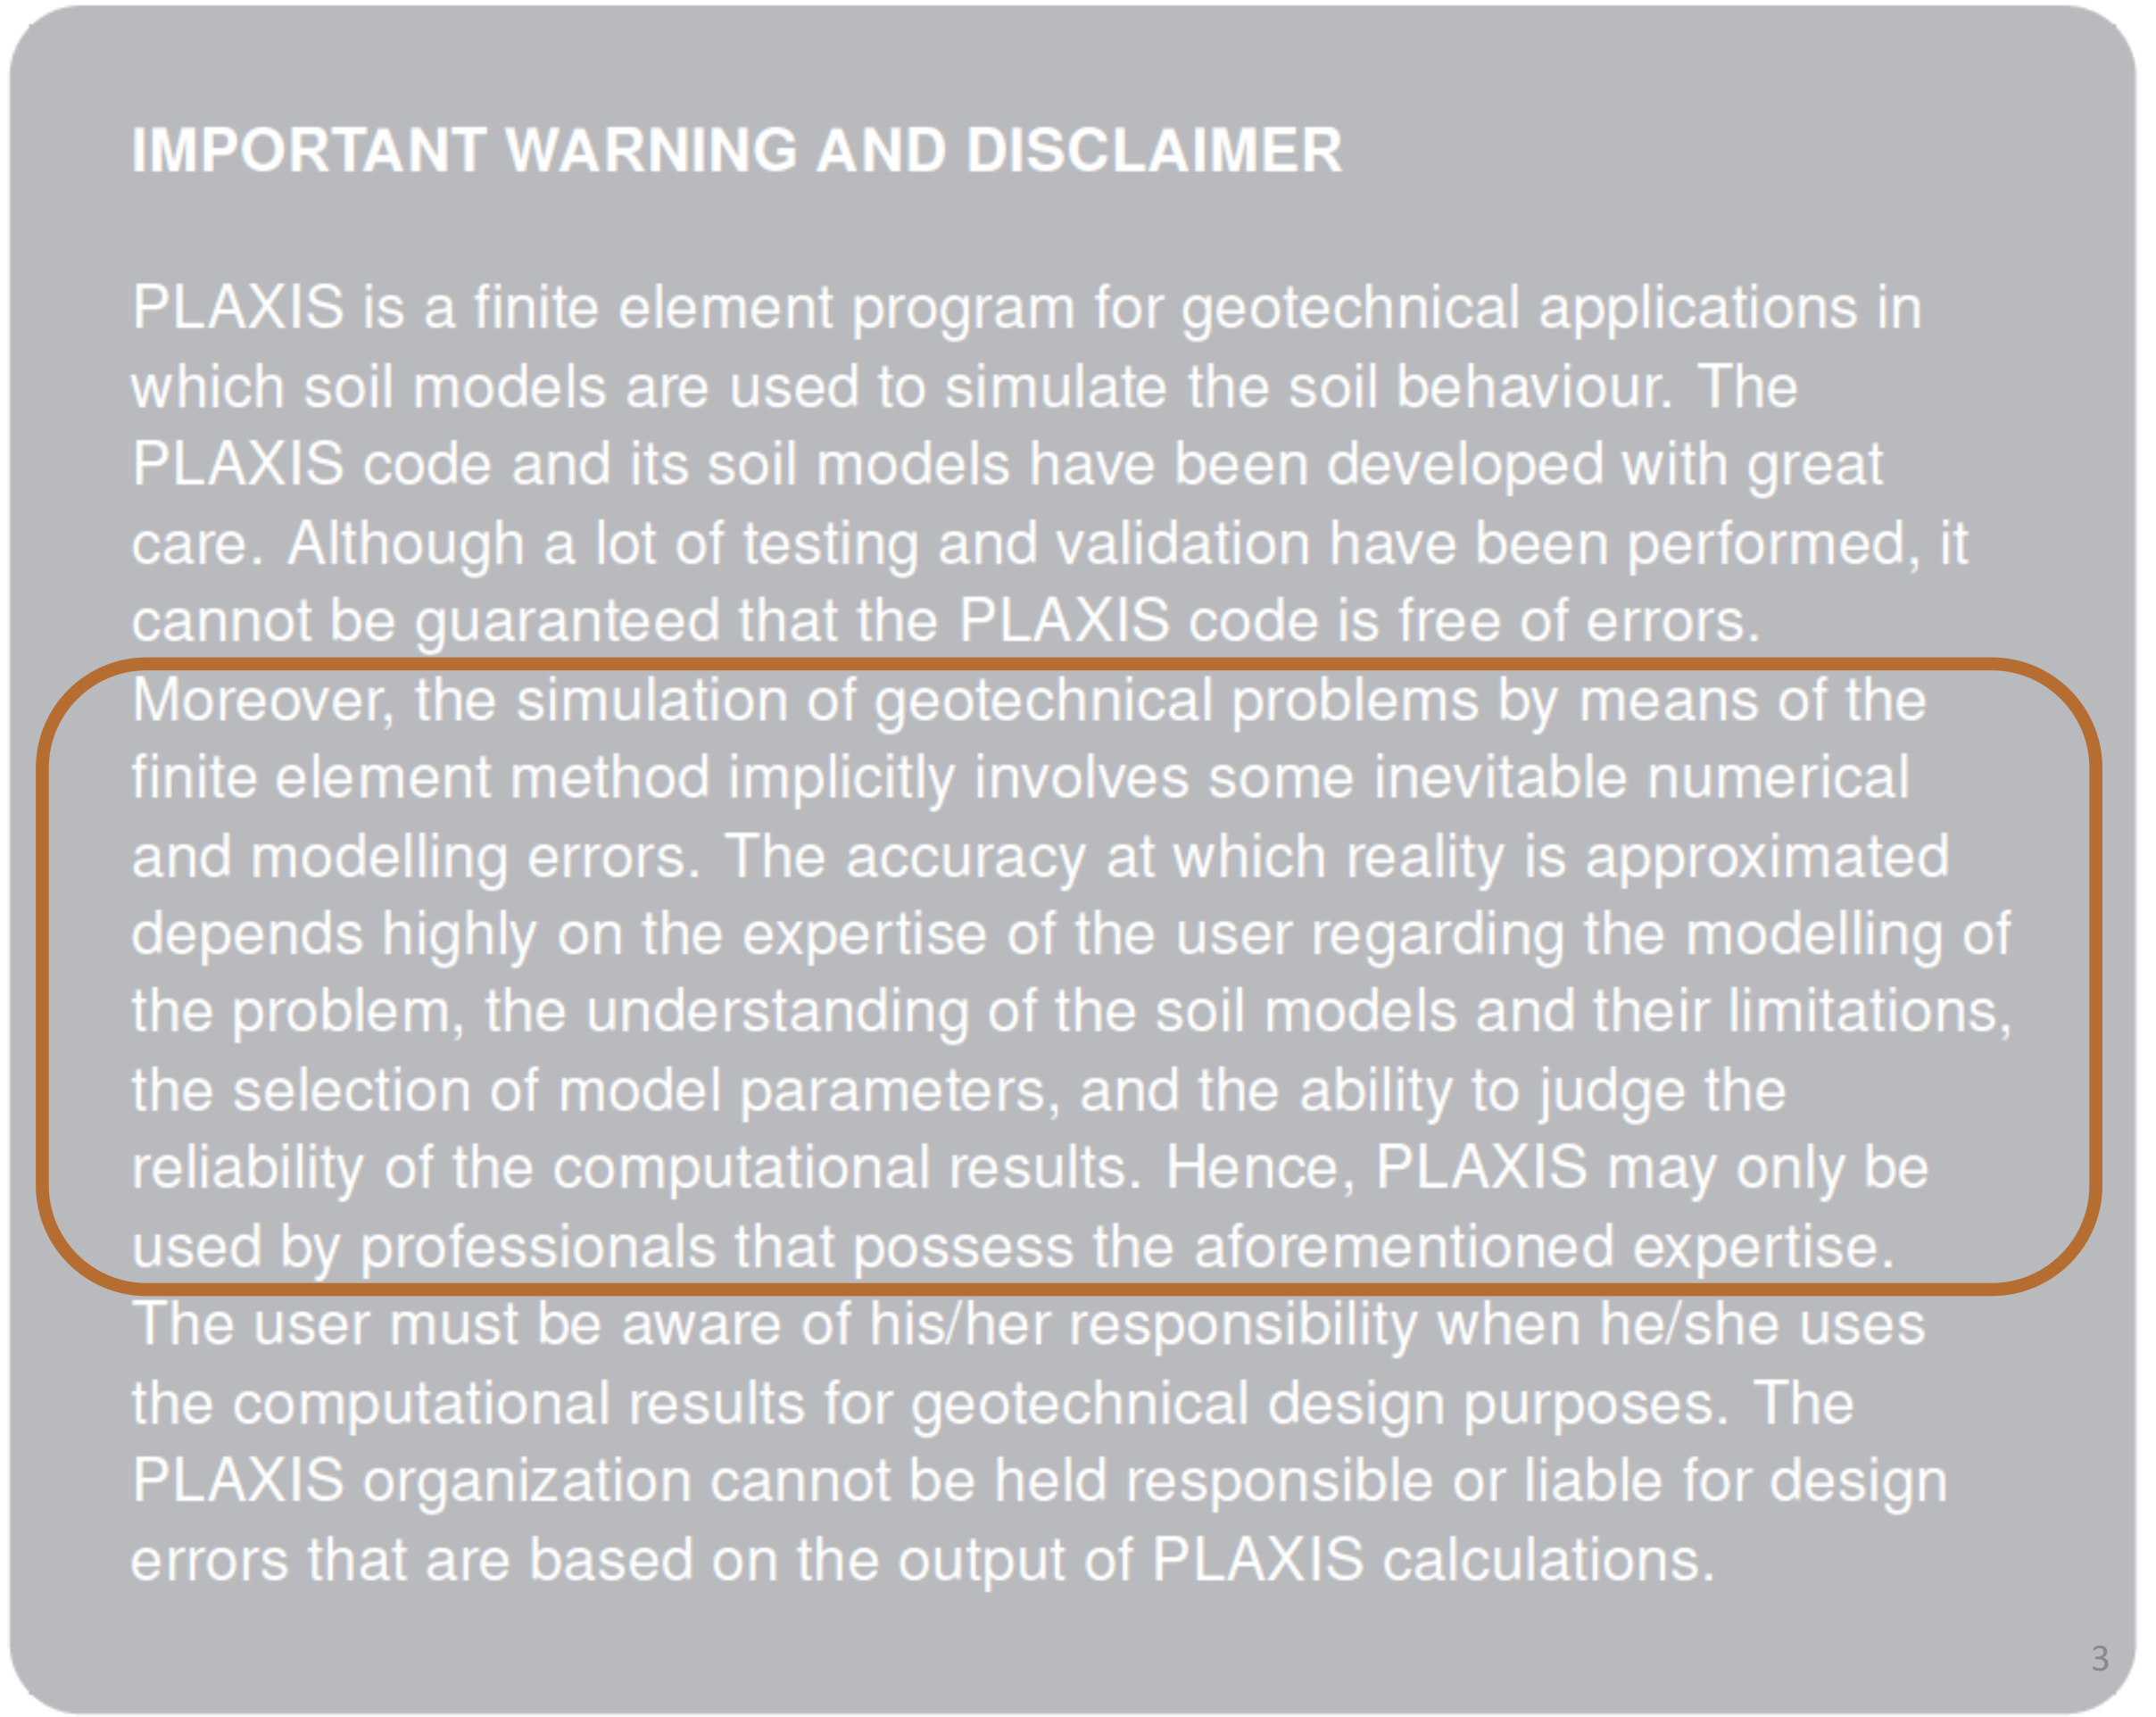
\includegraphics[width=0.85\textwidth]{figs/plaxis-disclaimer.png}
\end{figure}
\end{frame}

%------------------------------------------------
\begin{frame}
\frametitle{Consistent system of units}
\begin{figure}[ht]
	\centering
	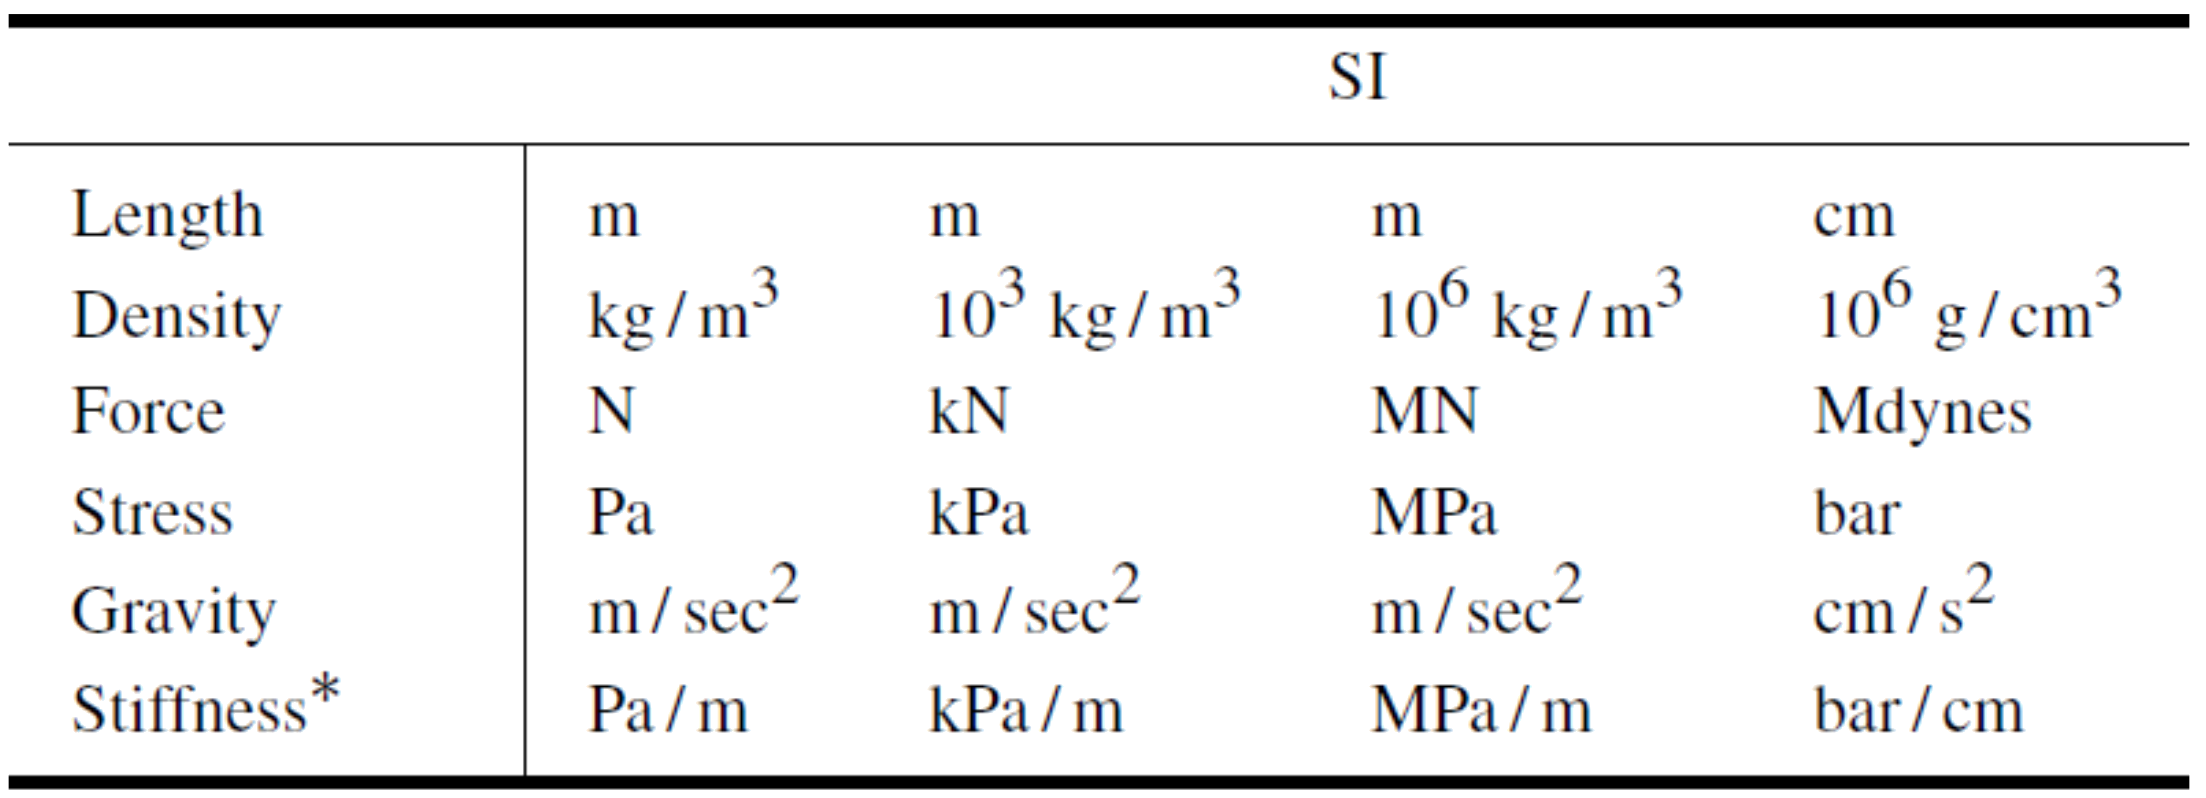
\includegraphics[width=0.85\textwidth]{figs/units.png}
\end{figure}
\end{frame}

%------------------------------------------------
\begin{frame}
\frametitle{Problem definition}
\mode<beamer>{
	\begin{figure}[ht]
		\centering
		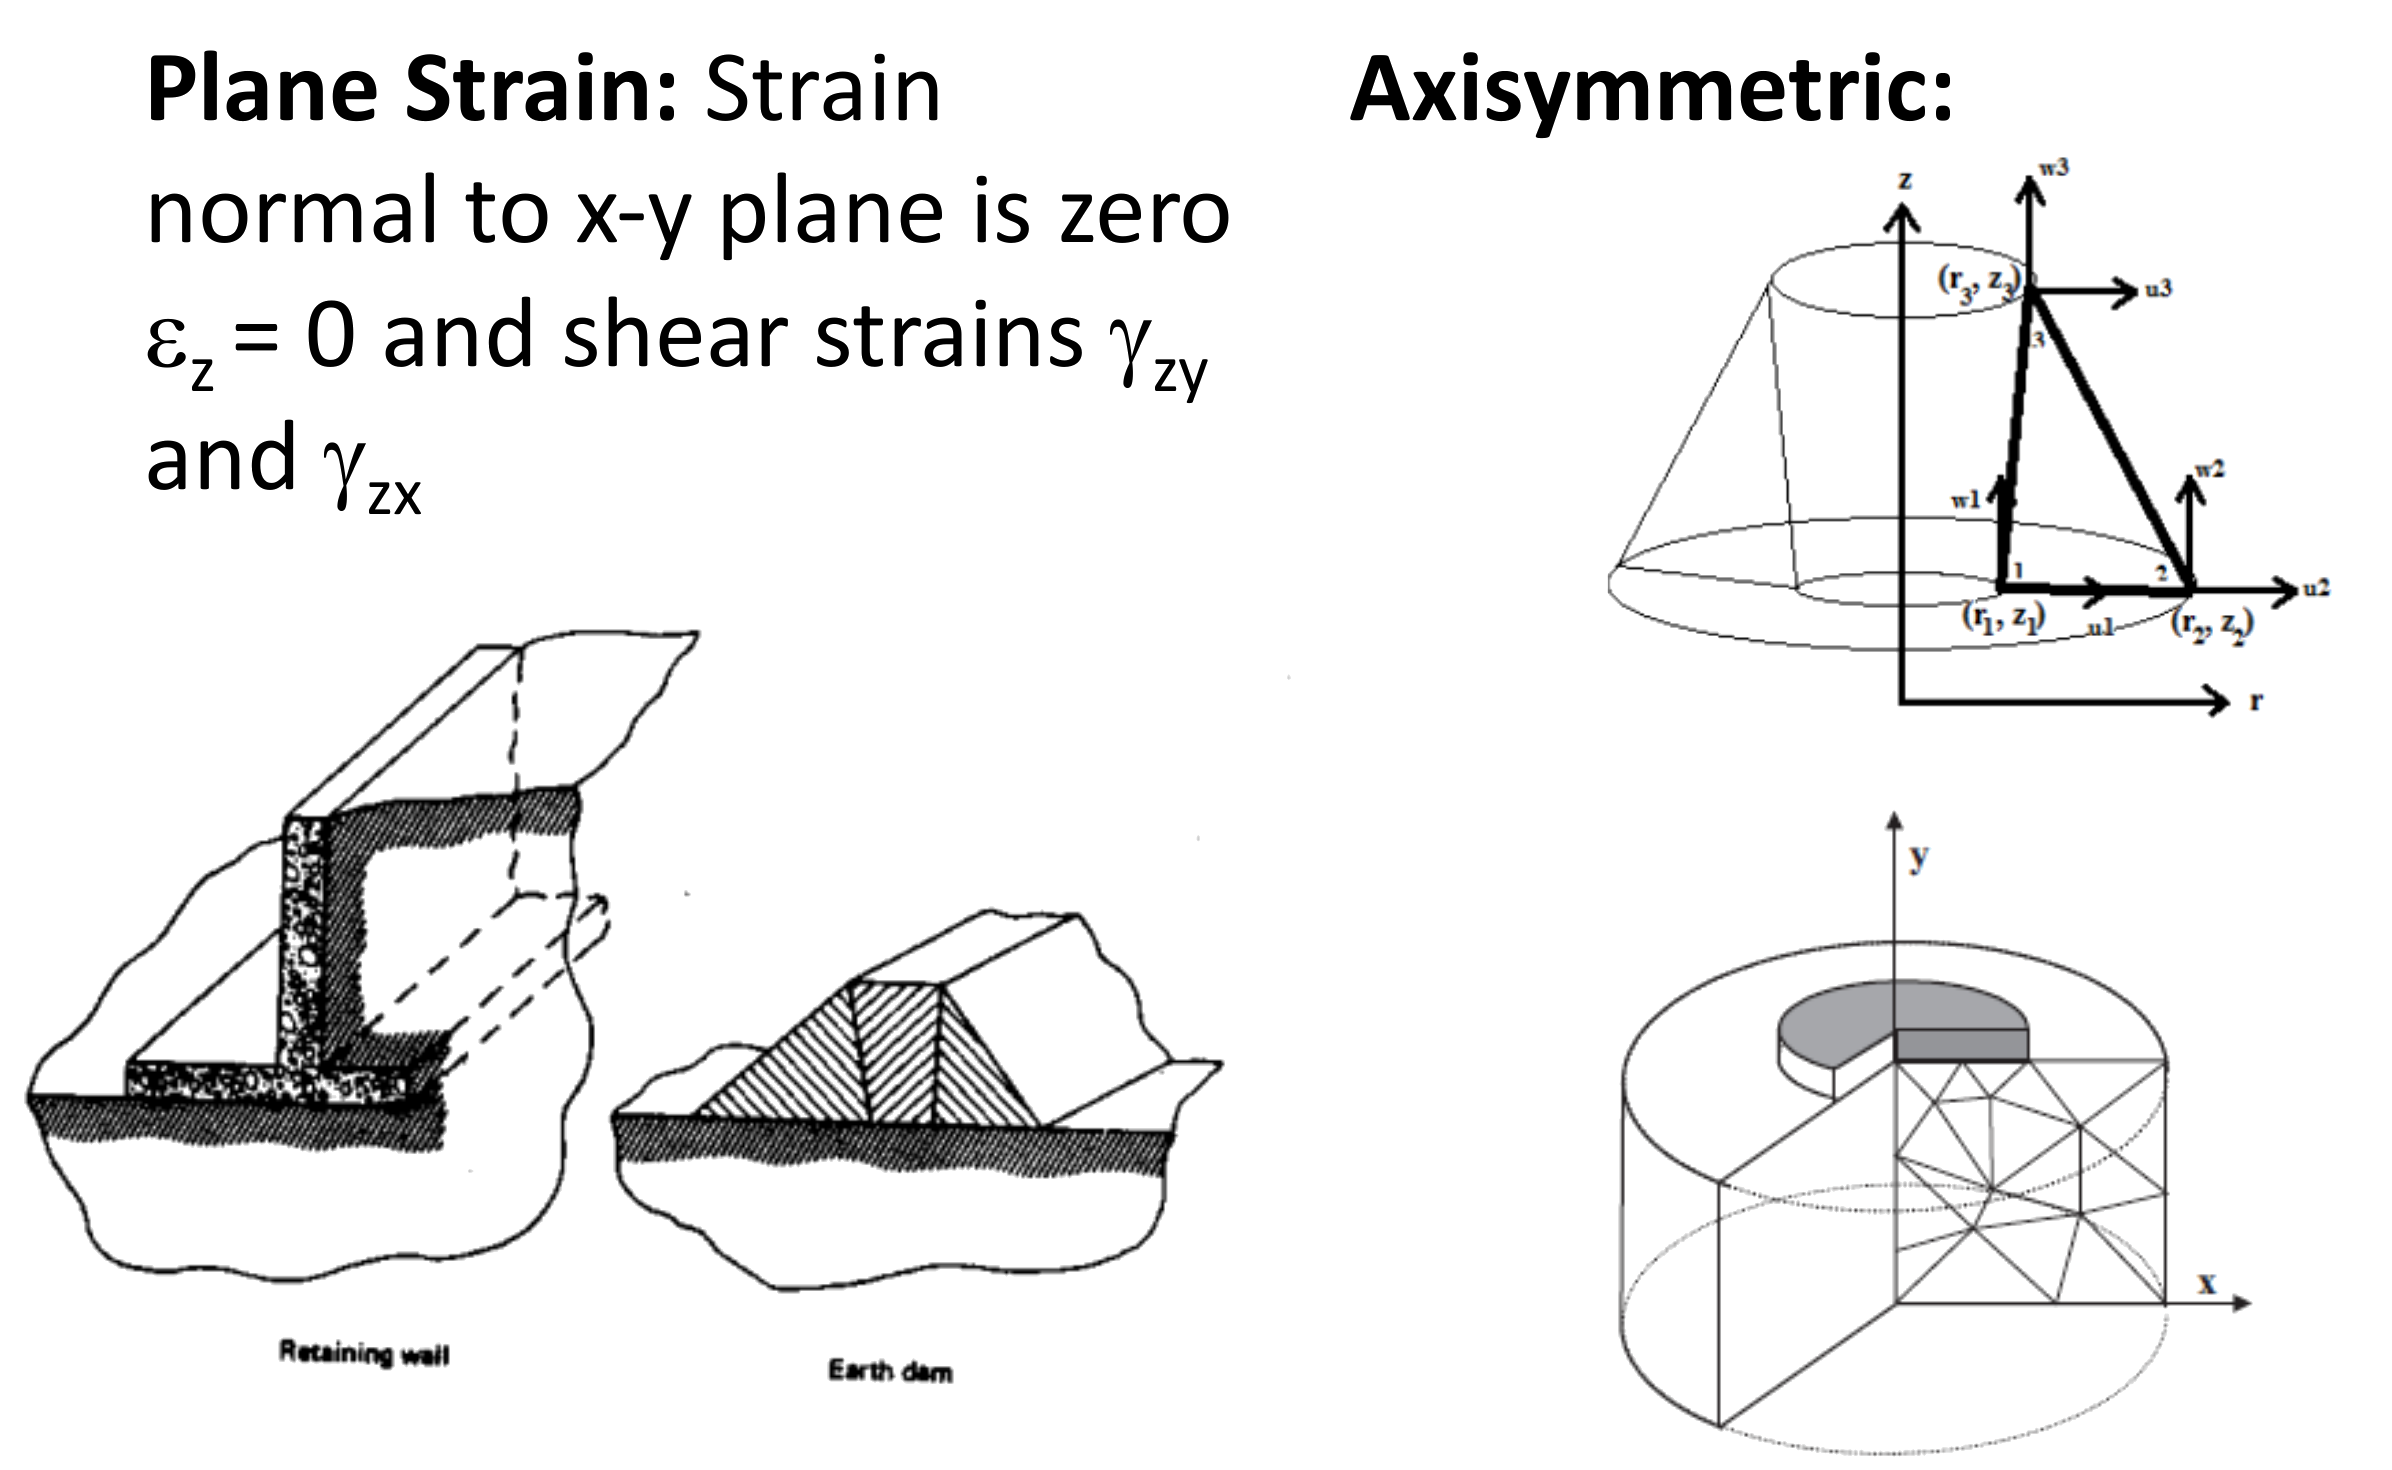
\includegraphics[width=0.85\textwidth]{figs/planestrain-axisymmetric.png}
		\caption*{Take advantage of symmetry}
	\end{figure}
}
\mode<handout>{
	\vspace{6cm}
}
\end{frame}

\subsection{Element types}
%------------------------------------------------
\begin{frame}
\frametitle{1D Finite Elements: Bar element}
Two node element with axial stiffness only (no flexural or shear
resistance).\mode<beamer>{Examples of this type of structure are cables, reinforcing bars.}
\begin{figure}[ht]
	\centering
	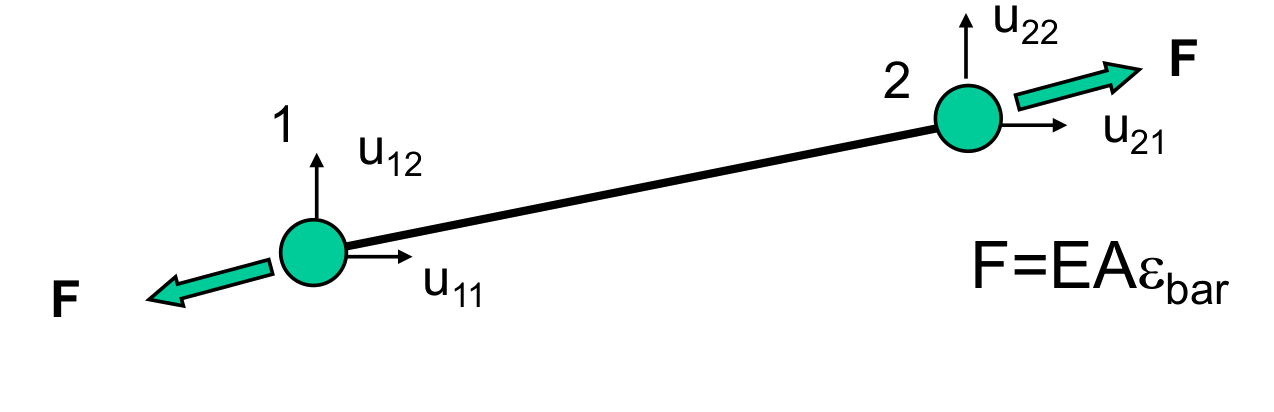
\includegraphics[width=0.65\textwidth]{figs/bar-element.png}
\end{figure}
\mode<handout>{
	\vspace{3cm}
}
\end{frame}

\note{
	\begin{enumerate}
		\item Node to Node: are springs that are used to model ties between two points. 
		\item It’s not recommended to draw geometry line at position where node-to-node anchor is to be placed. 
		\item It’s a 2 node elastic spring element with normal stiffness (Spring constant)
		\item Element can sustain both tensile forces (anchors) as well as compressive forces (struts).
		\item Fixed-End anchors:  Modelling of struts or props to sheet pile walls. 
	\end{enumerate}
}

\note{
	\begin{enumerate}
		\item Geogrids are slender structures with a normal stiffness but no bending stifness. 
		\item Geogrids can only sustain \textbf{Tensile forces} and no compression!
		\item Structures involving geotextiles. 
	\end{enumerate}
	\begin{figure}[ht]
		\centering
		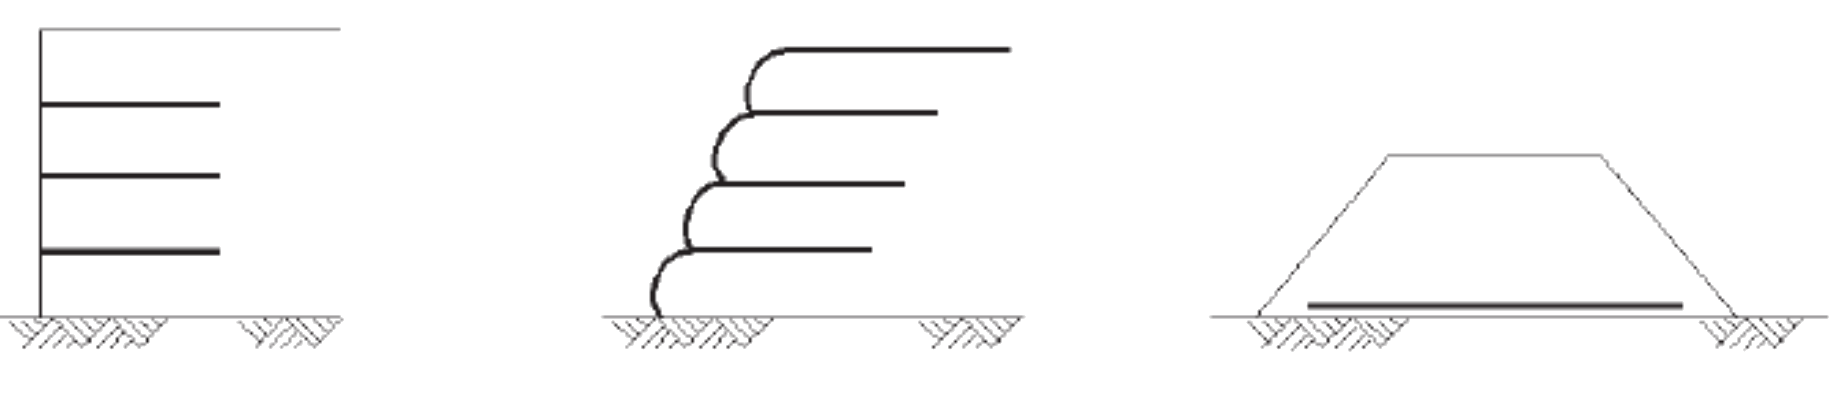
\includegraphics[width=0.85\textwidth]{figs/geogrids.png}
	\end{figure}
}

%------------------------------------------------
\begin{frame}
\frametitle{1D Finite Elements: Beam element}
two node structure element with axial and bending stiffness (no
transverse shear deformation). Three degrees of freedom for 2D beam element (1, 2
displacements and a moment). \mode<beamer>{Examples are sheet pile walls, structural foundation
	beams, structural facing for reinforced soil walls.}
\begin{figure}[h]
	\centering
	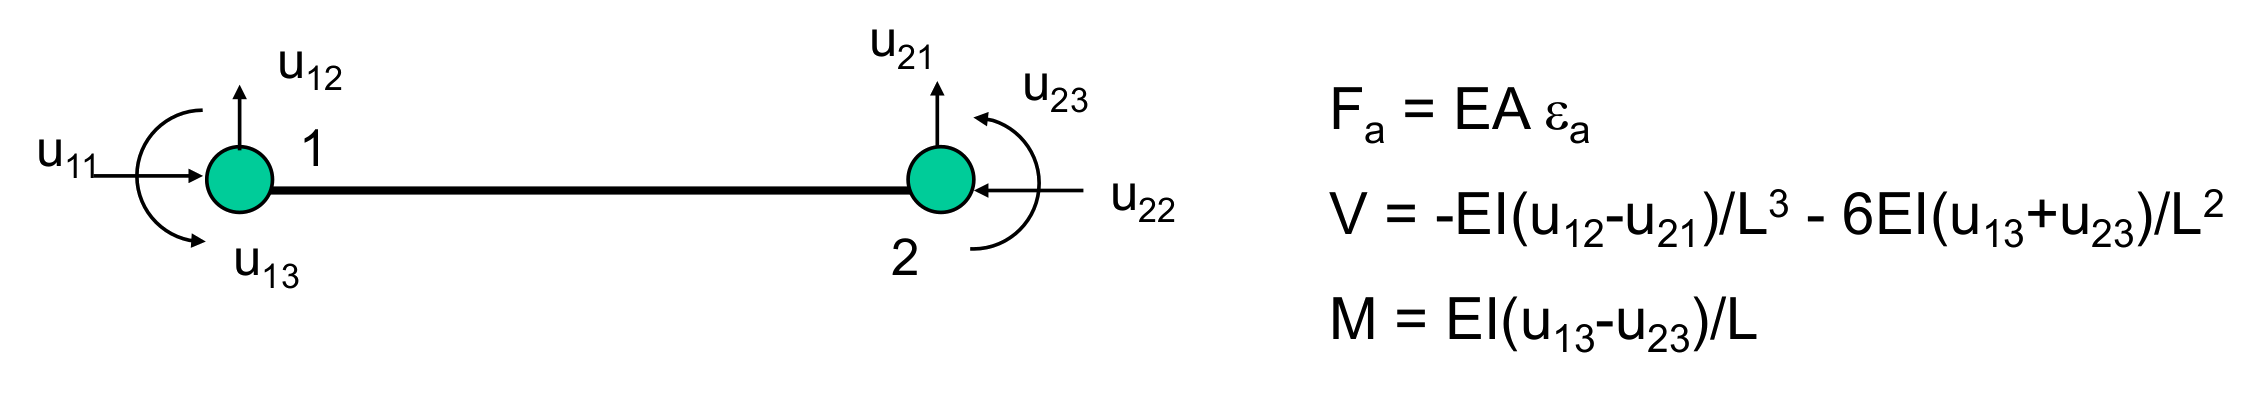
\includegraphics[width=0.75\textwidth]{figs/beam-element.png}
\end{figure}
\begin{figure}[h]
	\centering
	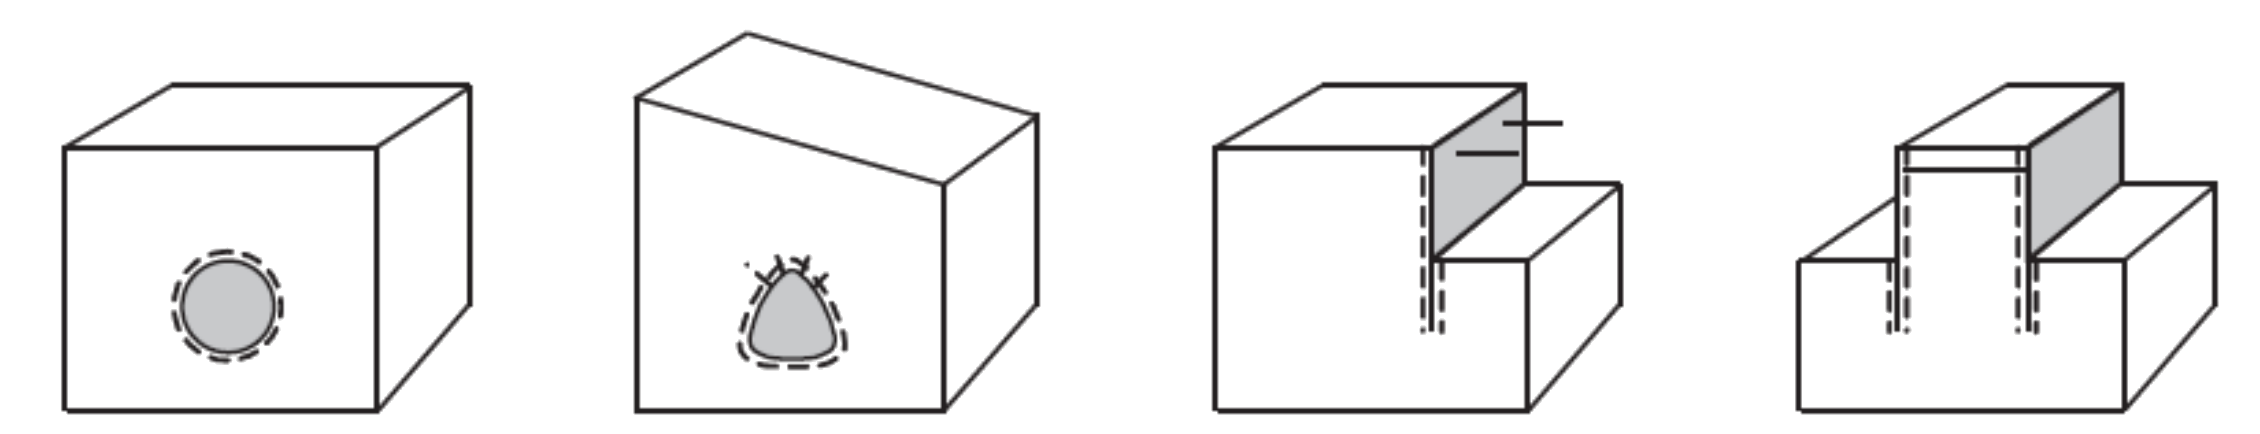
\includegraphics[width=0.75\textwidth]{figs/plate-elements.png}
\end{figure}
\end{frame}

%------------------------------------------------
\begin{frame}
\frametitle{2D plane-strain / axisymmetric elements}
\begin{figure}[ht]
	\centering
	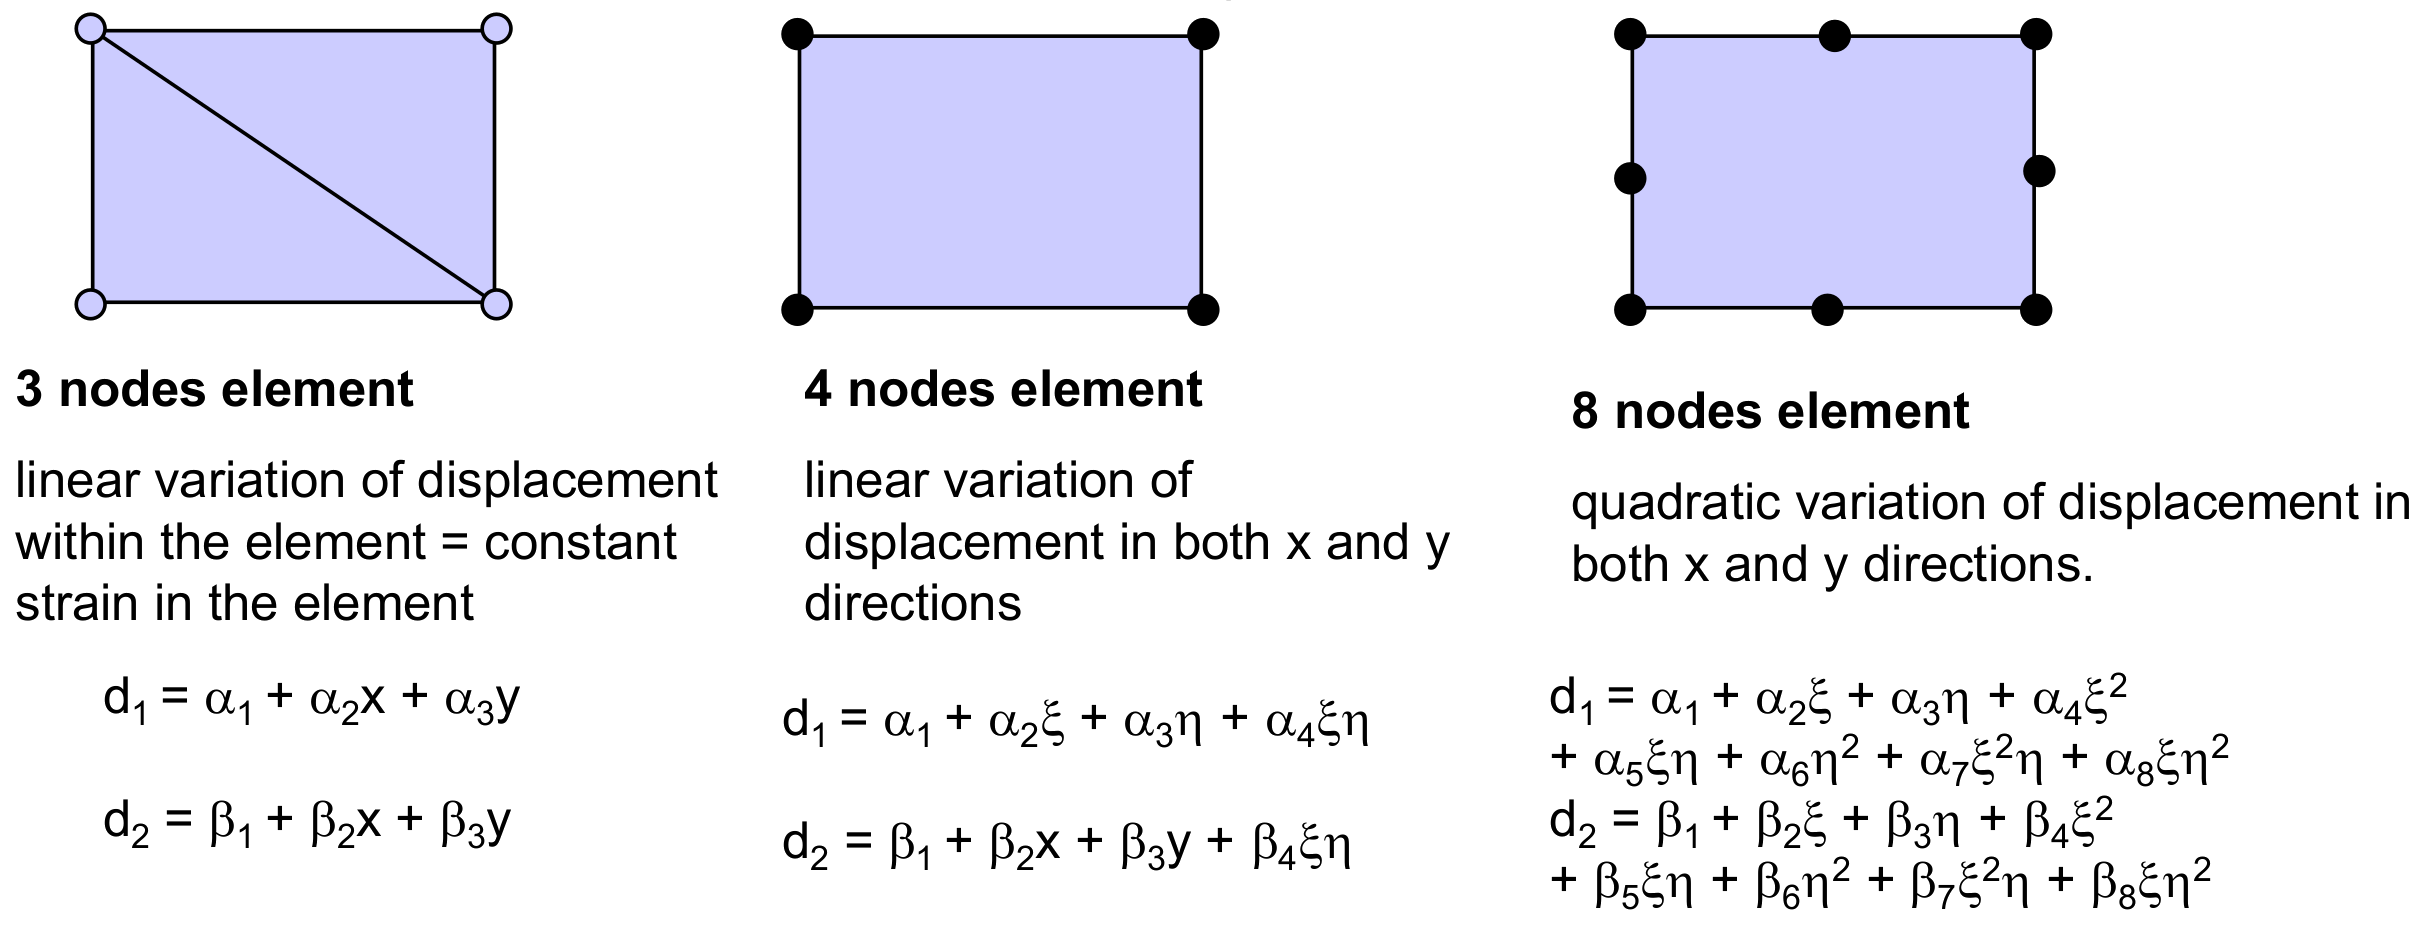
\includegraphics[width=\textwidth]{figs/2d-fe-elements.png}
\end{figure}
\end{frame}

%------------------------------------------------
\begin{frame}
\frametitle{2D/3D Finite elements}
\begin{figure}[ht]
	\centering
	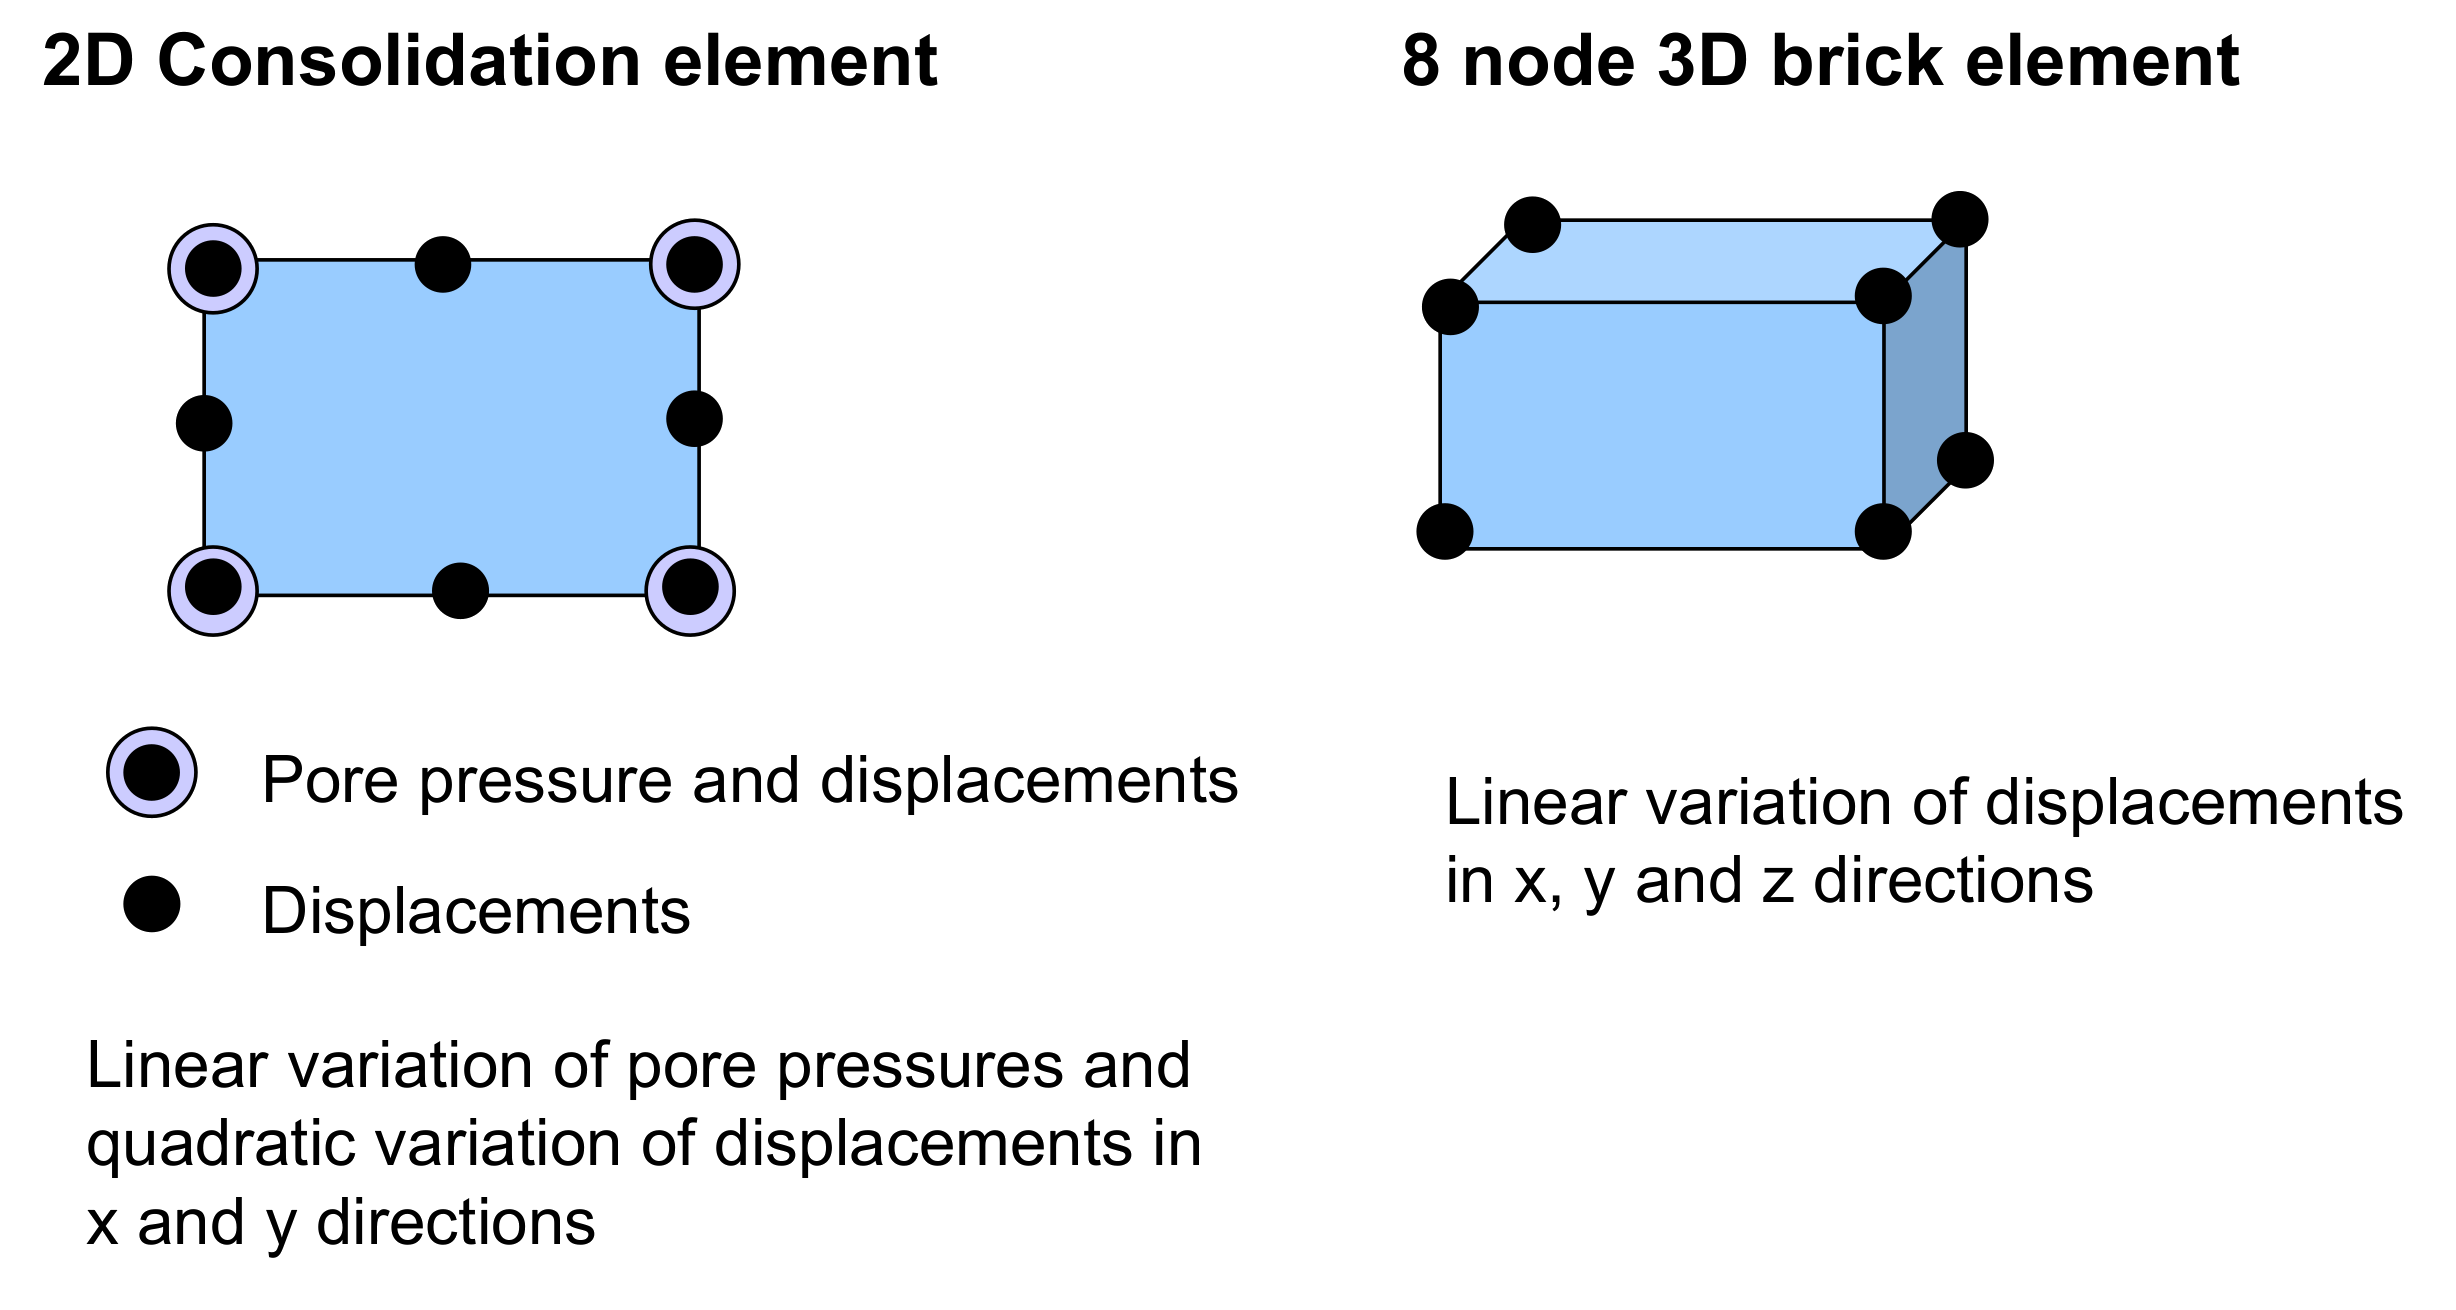
\includegraphics[width=\textwidth]{figs/2d-3d-elements.png}
\end{figure}
\end{frame}

%------------------------------------------------
\begin{frame}
\frametitle{Interface element}
\begin{figure}[ht]
	\centering
	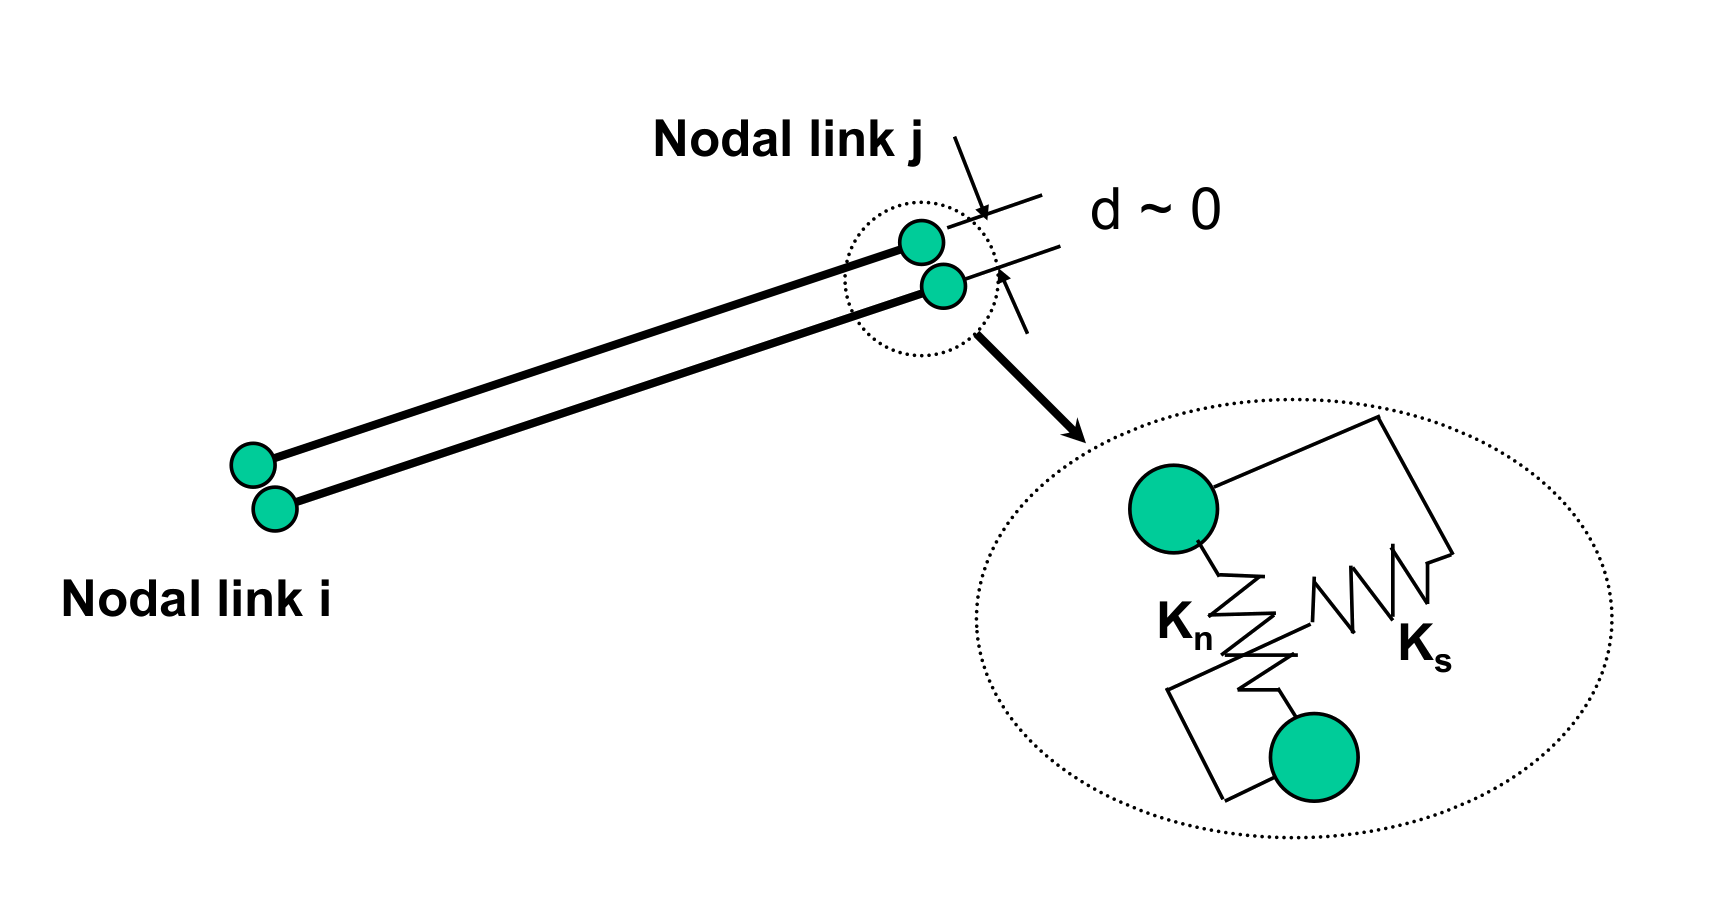
\includegraphics[width=0.5\textwidth]{figs/interface-element.png}
\end{figure}
\begin{figure}[ht]
	\centering
	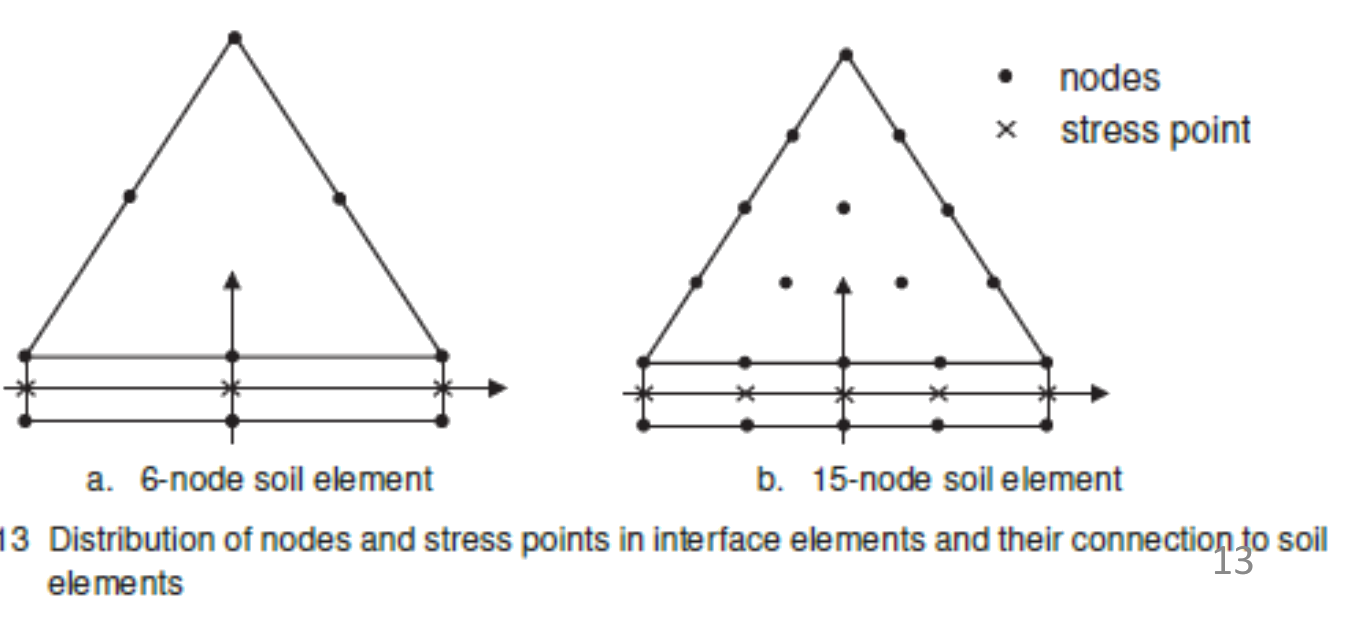
\includegraphics[width=0.6\textwidth]{figs/fe-interface.png}
	\caption*{Use a reduced strength at the interface}
\end{figure}
\end{frame}

\note{This element allows relative displacement between
elements. It is capable to model soil/structure interface conditions, shear planes
within a soil mass. The element is ‘fictitious’ four node element made up of two
independent nodal links. Each link consists of two nodes connected by a normal
and shear spring as shown below. The stiffness of the springs can be non-linear,
modelling frictional slip behaviour. The thickness of the element is assumed to be
negligibles}

%------------------------------------------------
\begin{frame}
\frametitle{Interface elements for Soil Structure Interactions}
\begin{figure}[ht]
	\centering
	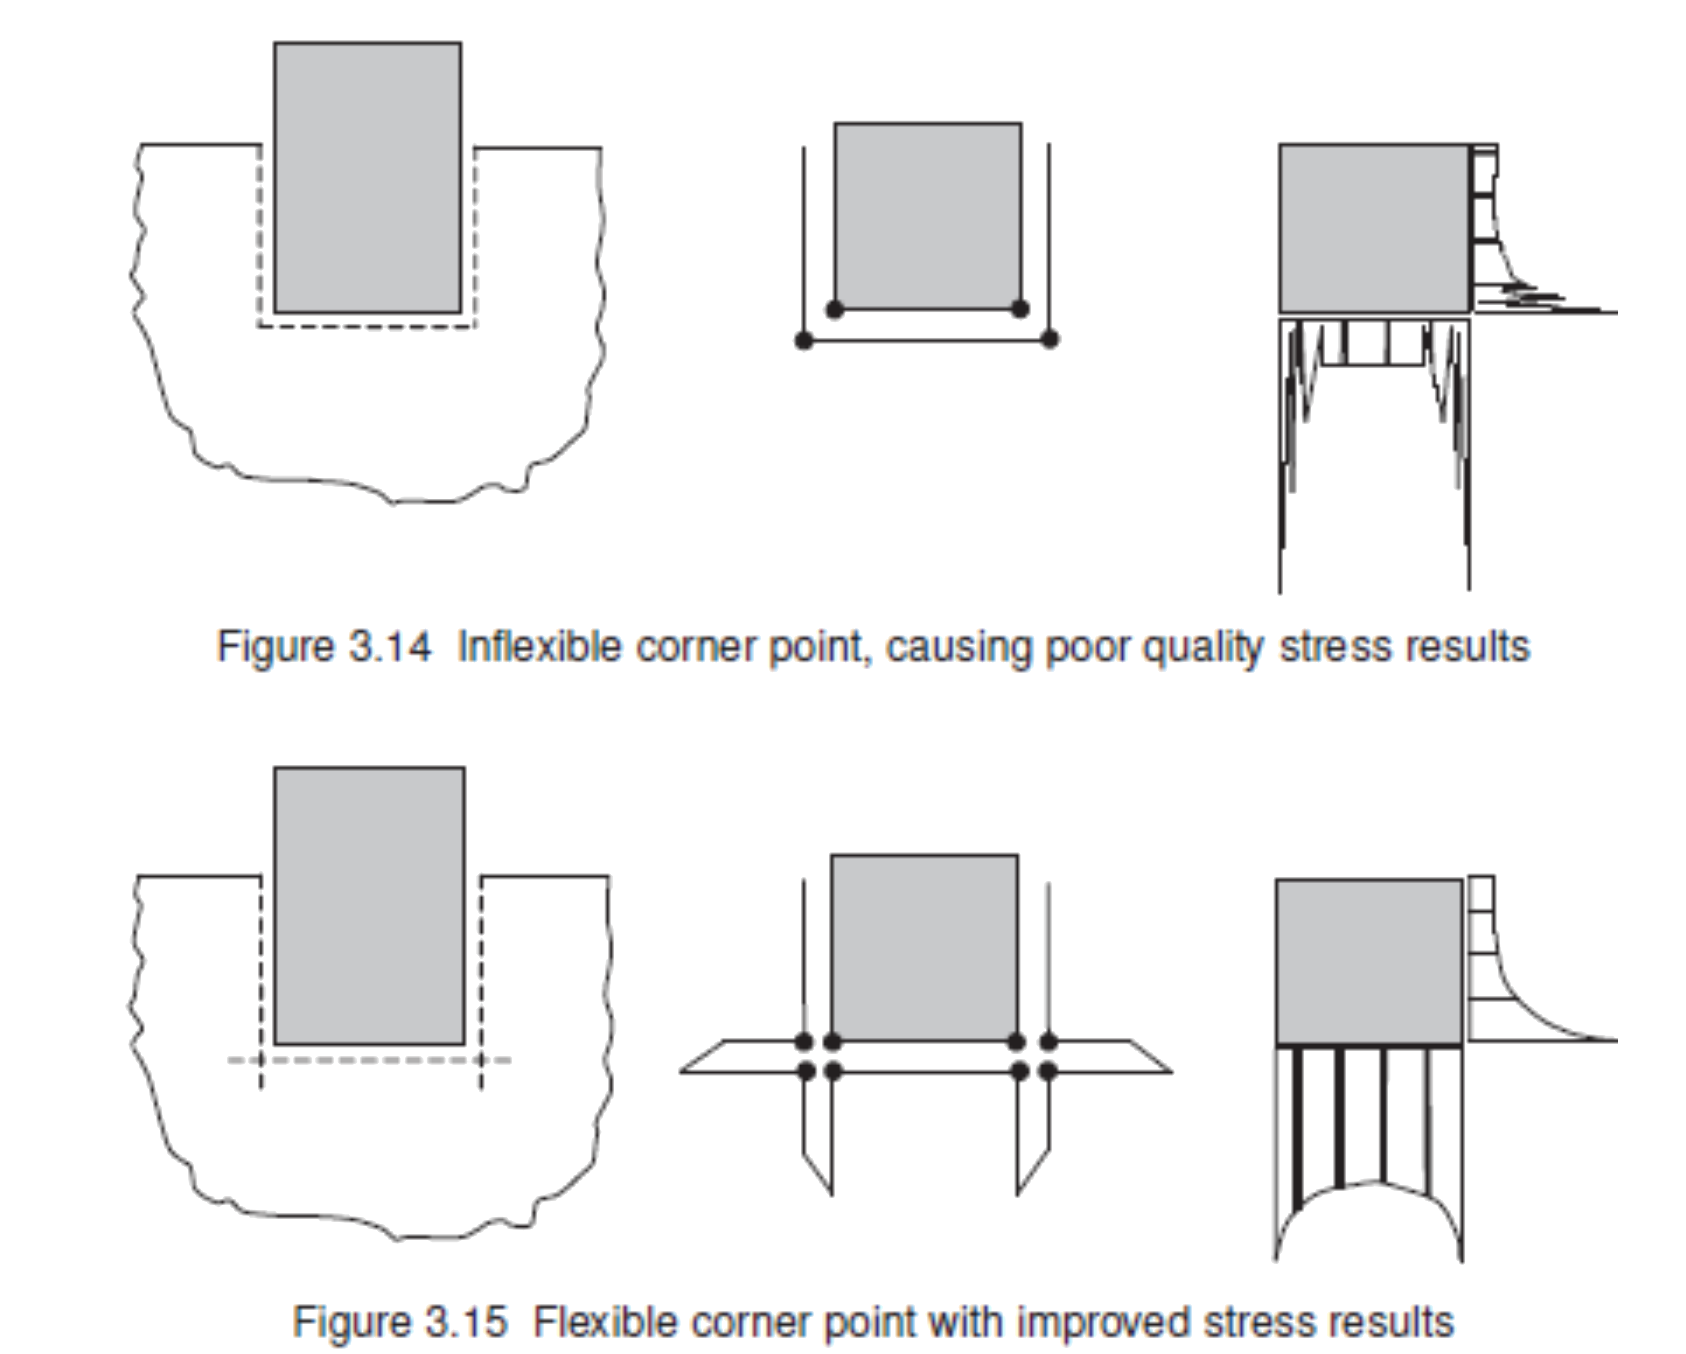
\includegraphics[width=0.65\textwidth]{figs/interface-ssi.png}
\end{figure}
\end{frame}

\subsection{Discretization}
%------------------------------------------------
\begin{frame}
\frametitle{FE discretization}
\begin{figure}[ht]
	\centering
	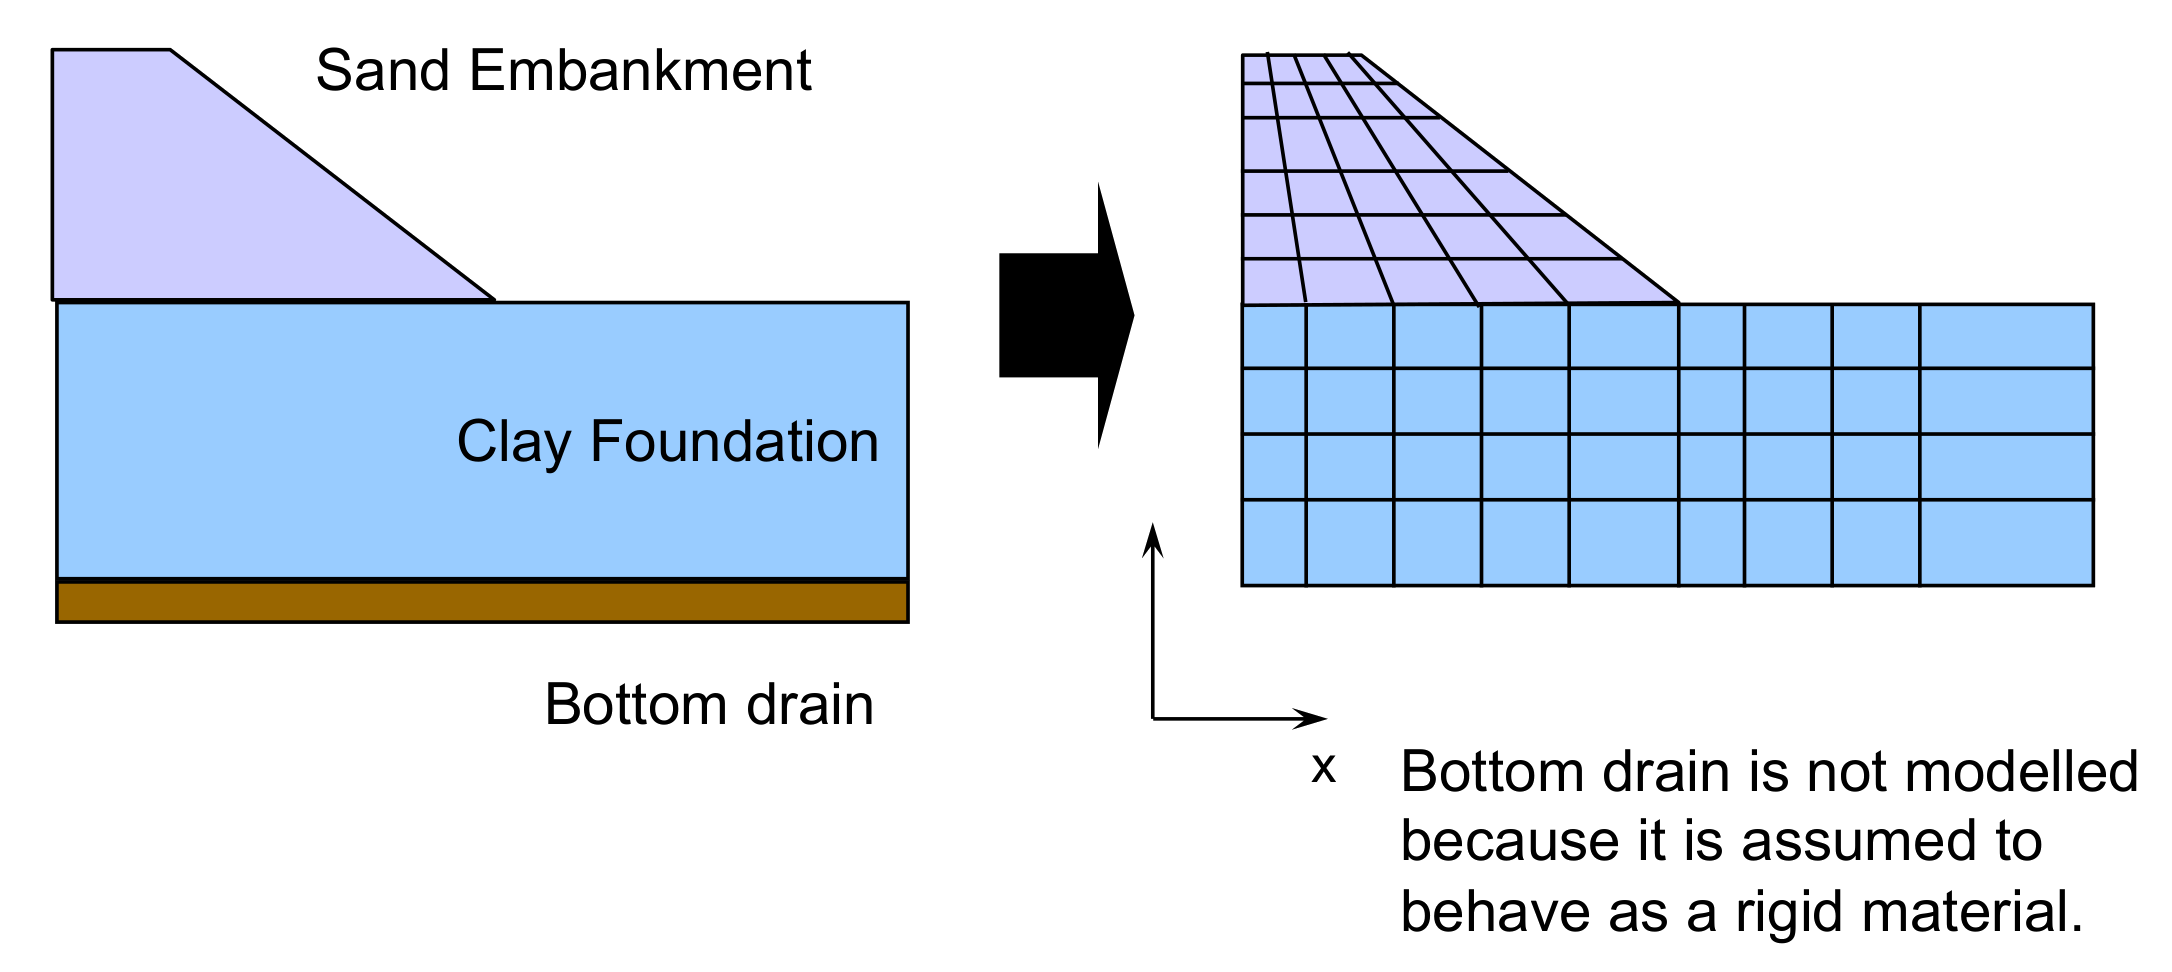
\includegraphics[width=\textwidth]{figs/discretization.png}
\end{figure}
\end{frame}

%------------------------------------------------
\begin{frame}
\frametitle{FE discretization}
\begin{figure}[ht]
	\centering
	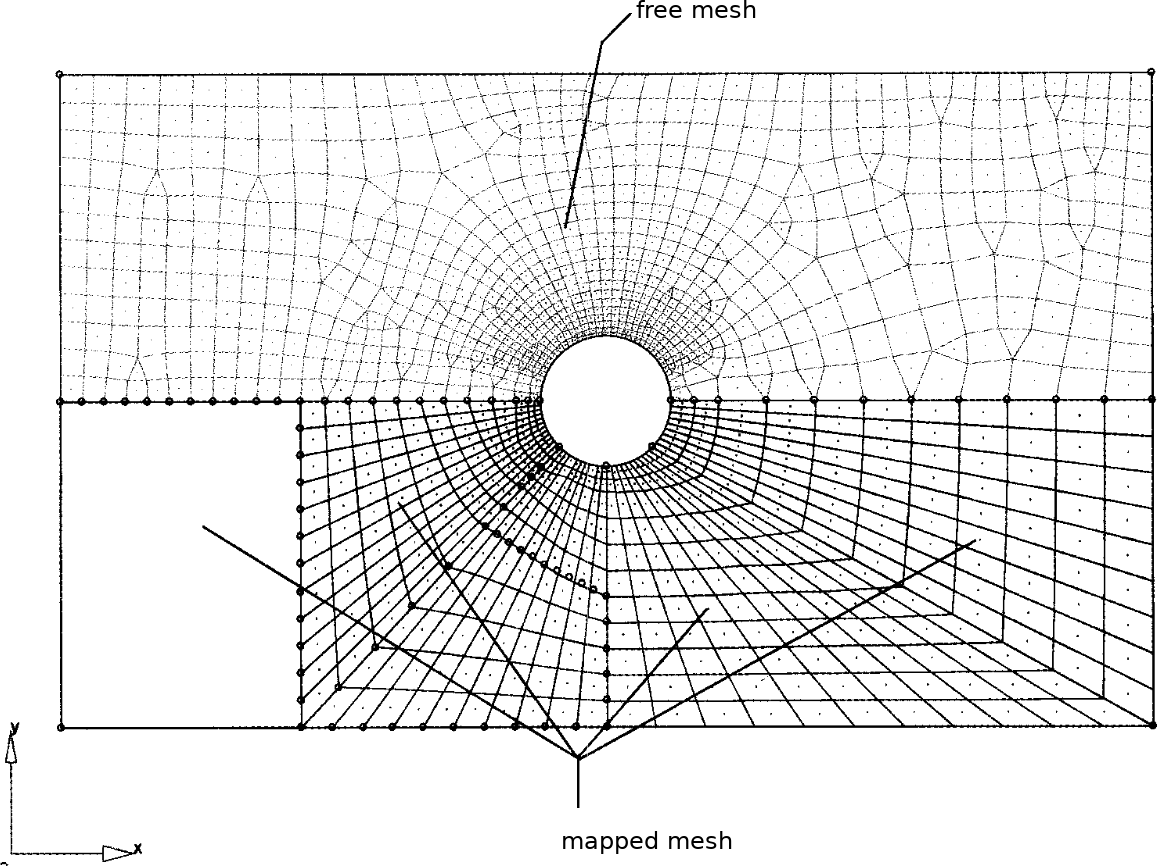
\includegraphics[width=0.8\textwidth]{figs/mesh-discretization.png}
\end{figure}
\end{frame}

\note{
	There are many algorithms to generate mesh for a given object. The top part of the geometry is a
	mesh generated by ``\textit{free meshing}'', in which elements are generated automatically with triangles
	and quadrilaterals within the whole domain. The bottom part of the geometry is a mesh generated by
	``\textit{mapped meshing}'', in which quadrilateral elements are placed in subzones with a more regular
	manner. The mesh density is also more controlled.\\
	
	Some elements generated in the previous figure show that the interior nodes are shared by
	more than one element. The number of elements that share a node is called valence. The
	ideal valence of interior nodes for quadrilaterals is four to achieve the optimum interior angle
	of 90 degrees. For triangles, it is six. After a mesh is generated, it is ideal to clean up the
	mesh.
}

%------------------------------------------------
\begin{frame}
\frametitle{FE discretization}
	
\noindent
\fboxsep=0pt
\noindent
\begin{minipage}[t]{0.49\linewidth}
	\begin{figure}
		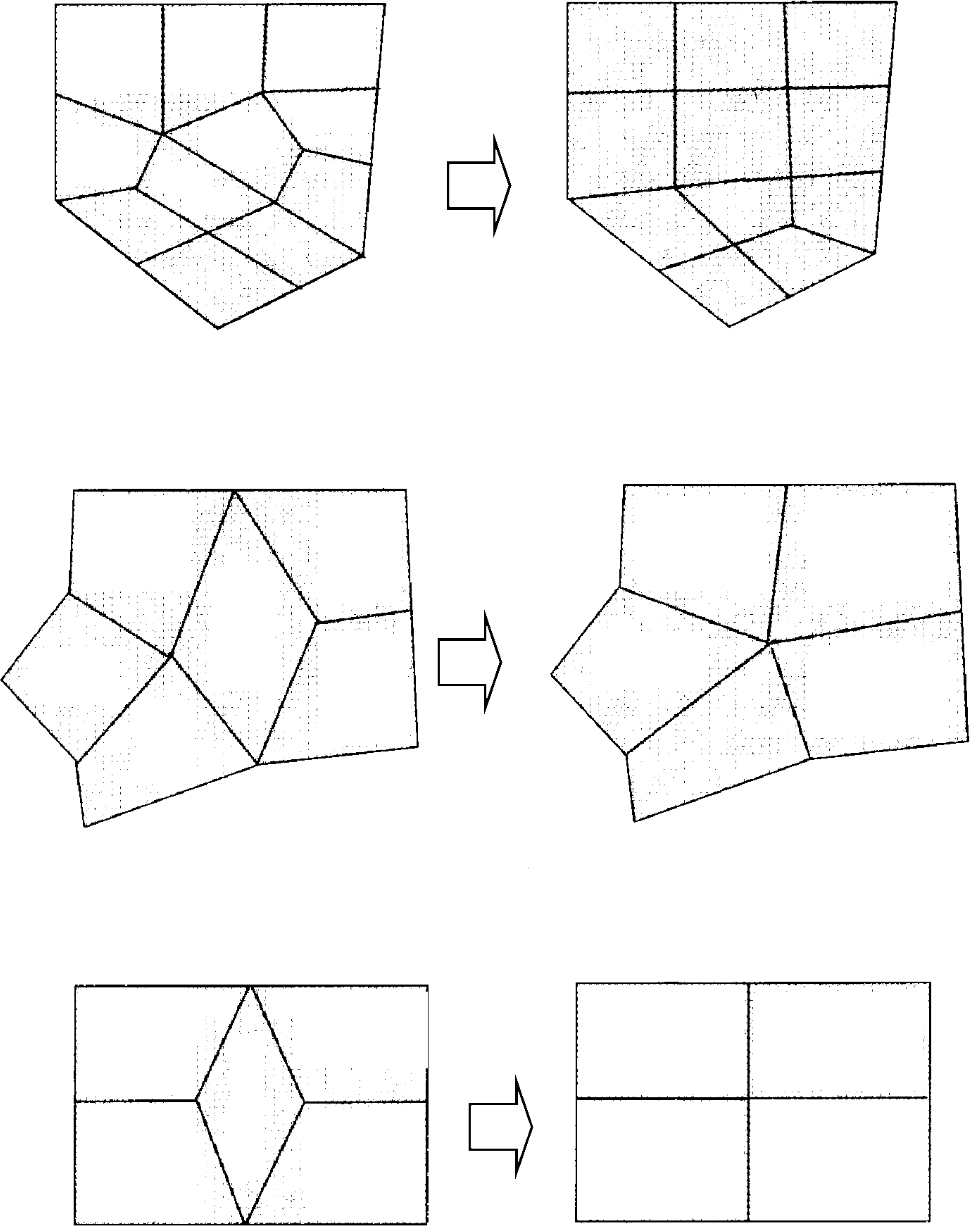
\includegraphics[width=\textwidth]{figs/element-repair.png}
	\end{figure}
\end{minipage}%
\hfill%
\begin{minipage}[t]{0.49\linewidth}
	\begin{enumerate}
		\item Node valence less or equal to two and greater than or equal to
		six should be eliminated.
		\item The number of nodes with valence of three or five should be
		minimized.
		\item Angles greater than 160 degrees should be eliminated.
		\item The aspect ratio should be less than 3 for stress analysis and
		10 for displacement analysis.
	\end{enumerate}
\end{minipage}	
\end{frame}


%------------------------------------------------
\begin{frame}
\frametitle{FE discretization}
\begin{figure}[ht]
	\centering
	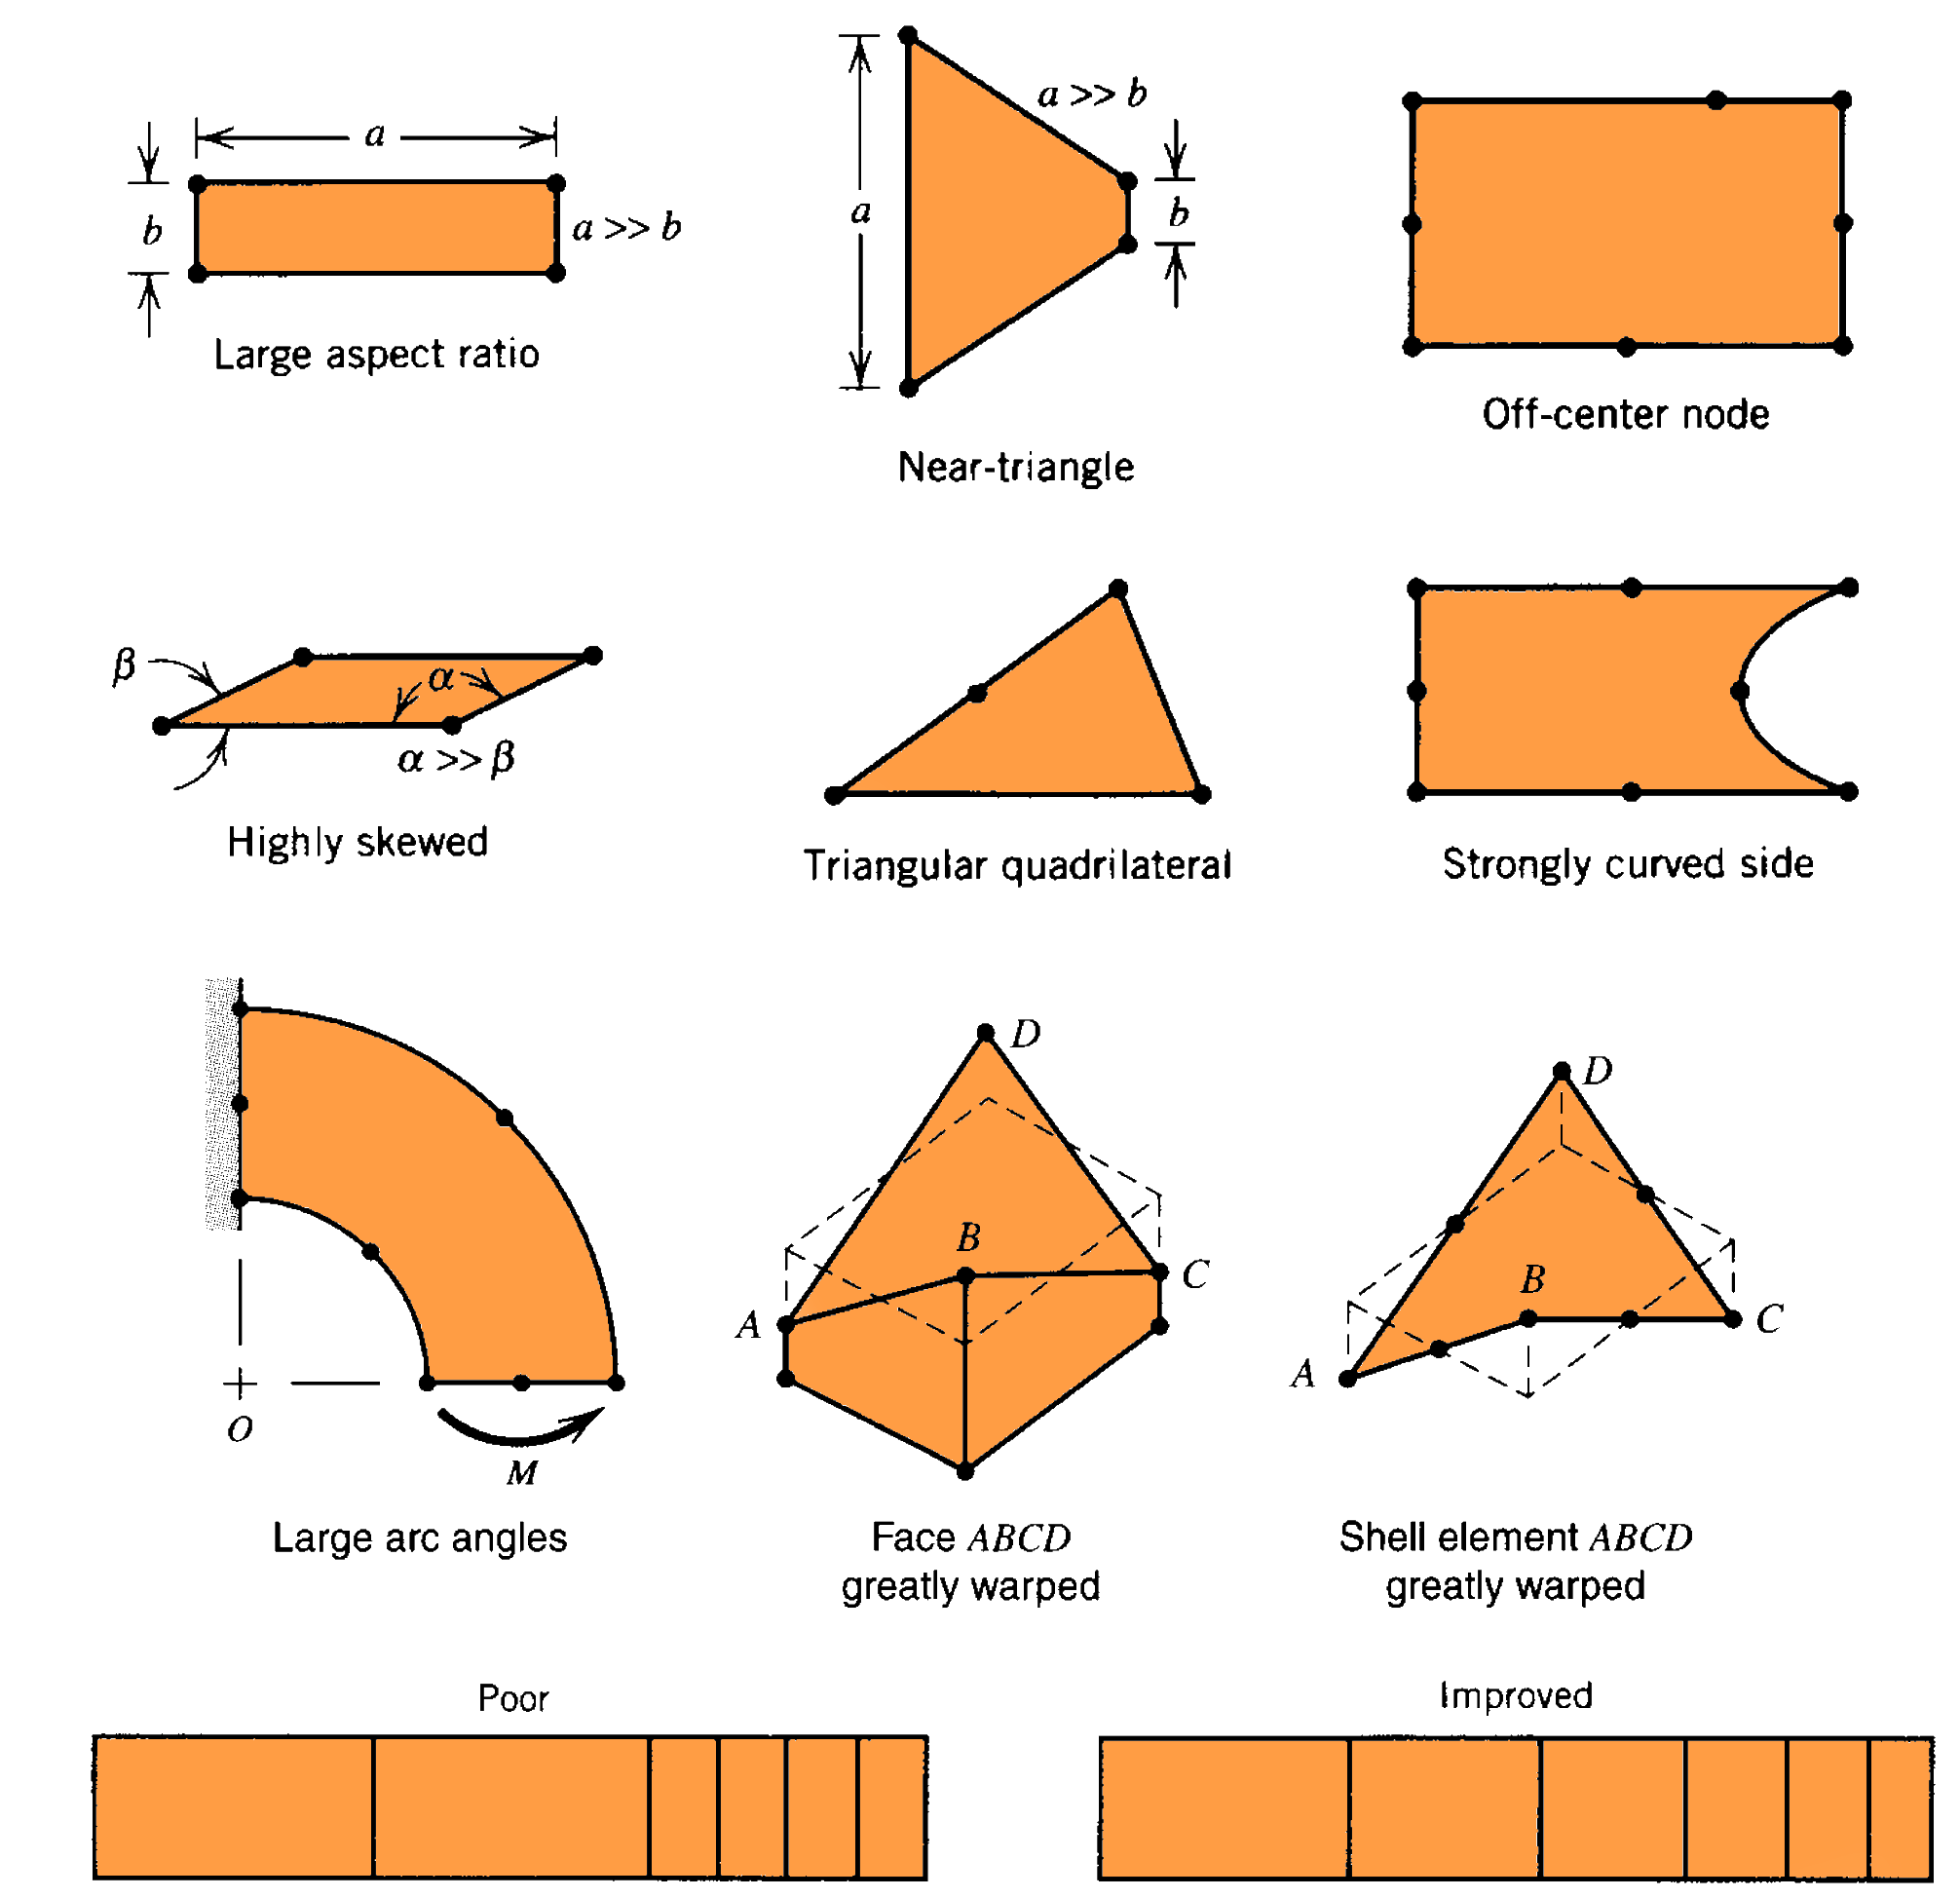
\includegraphics[width=0.8\textwidth]{figs/acceptable-discretization.png}
\end{figure}
\end{frame}

%------------------------------------------------
\begin{frame}
\frametitle{FE discretization}
\mode<beamer>{
	\begin{figure}[ht]
		\centering
		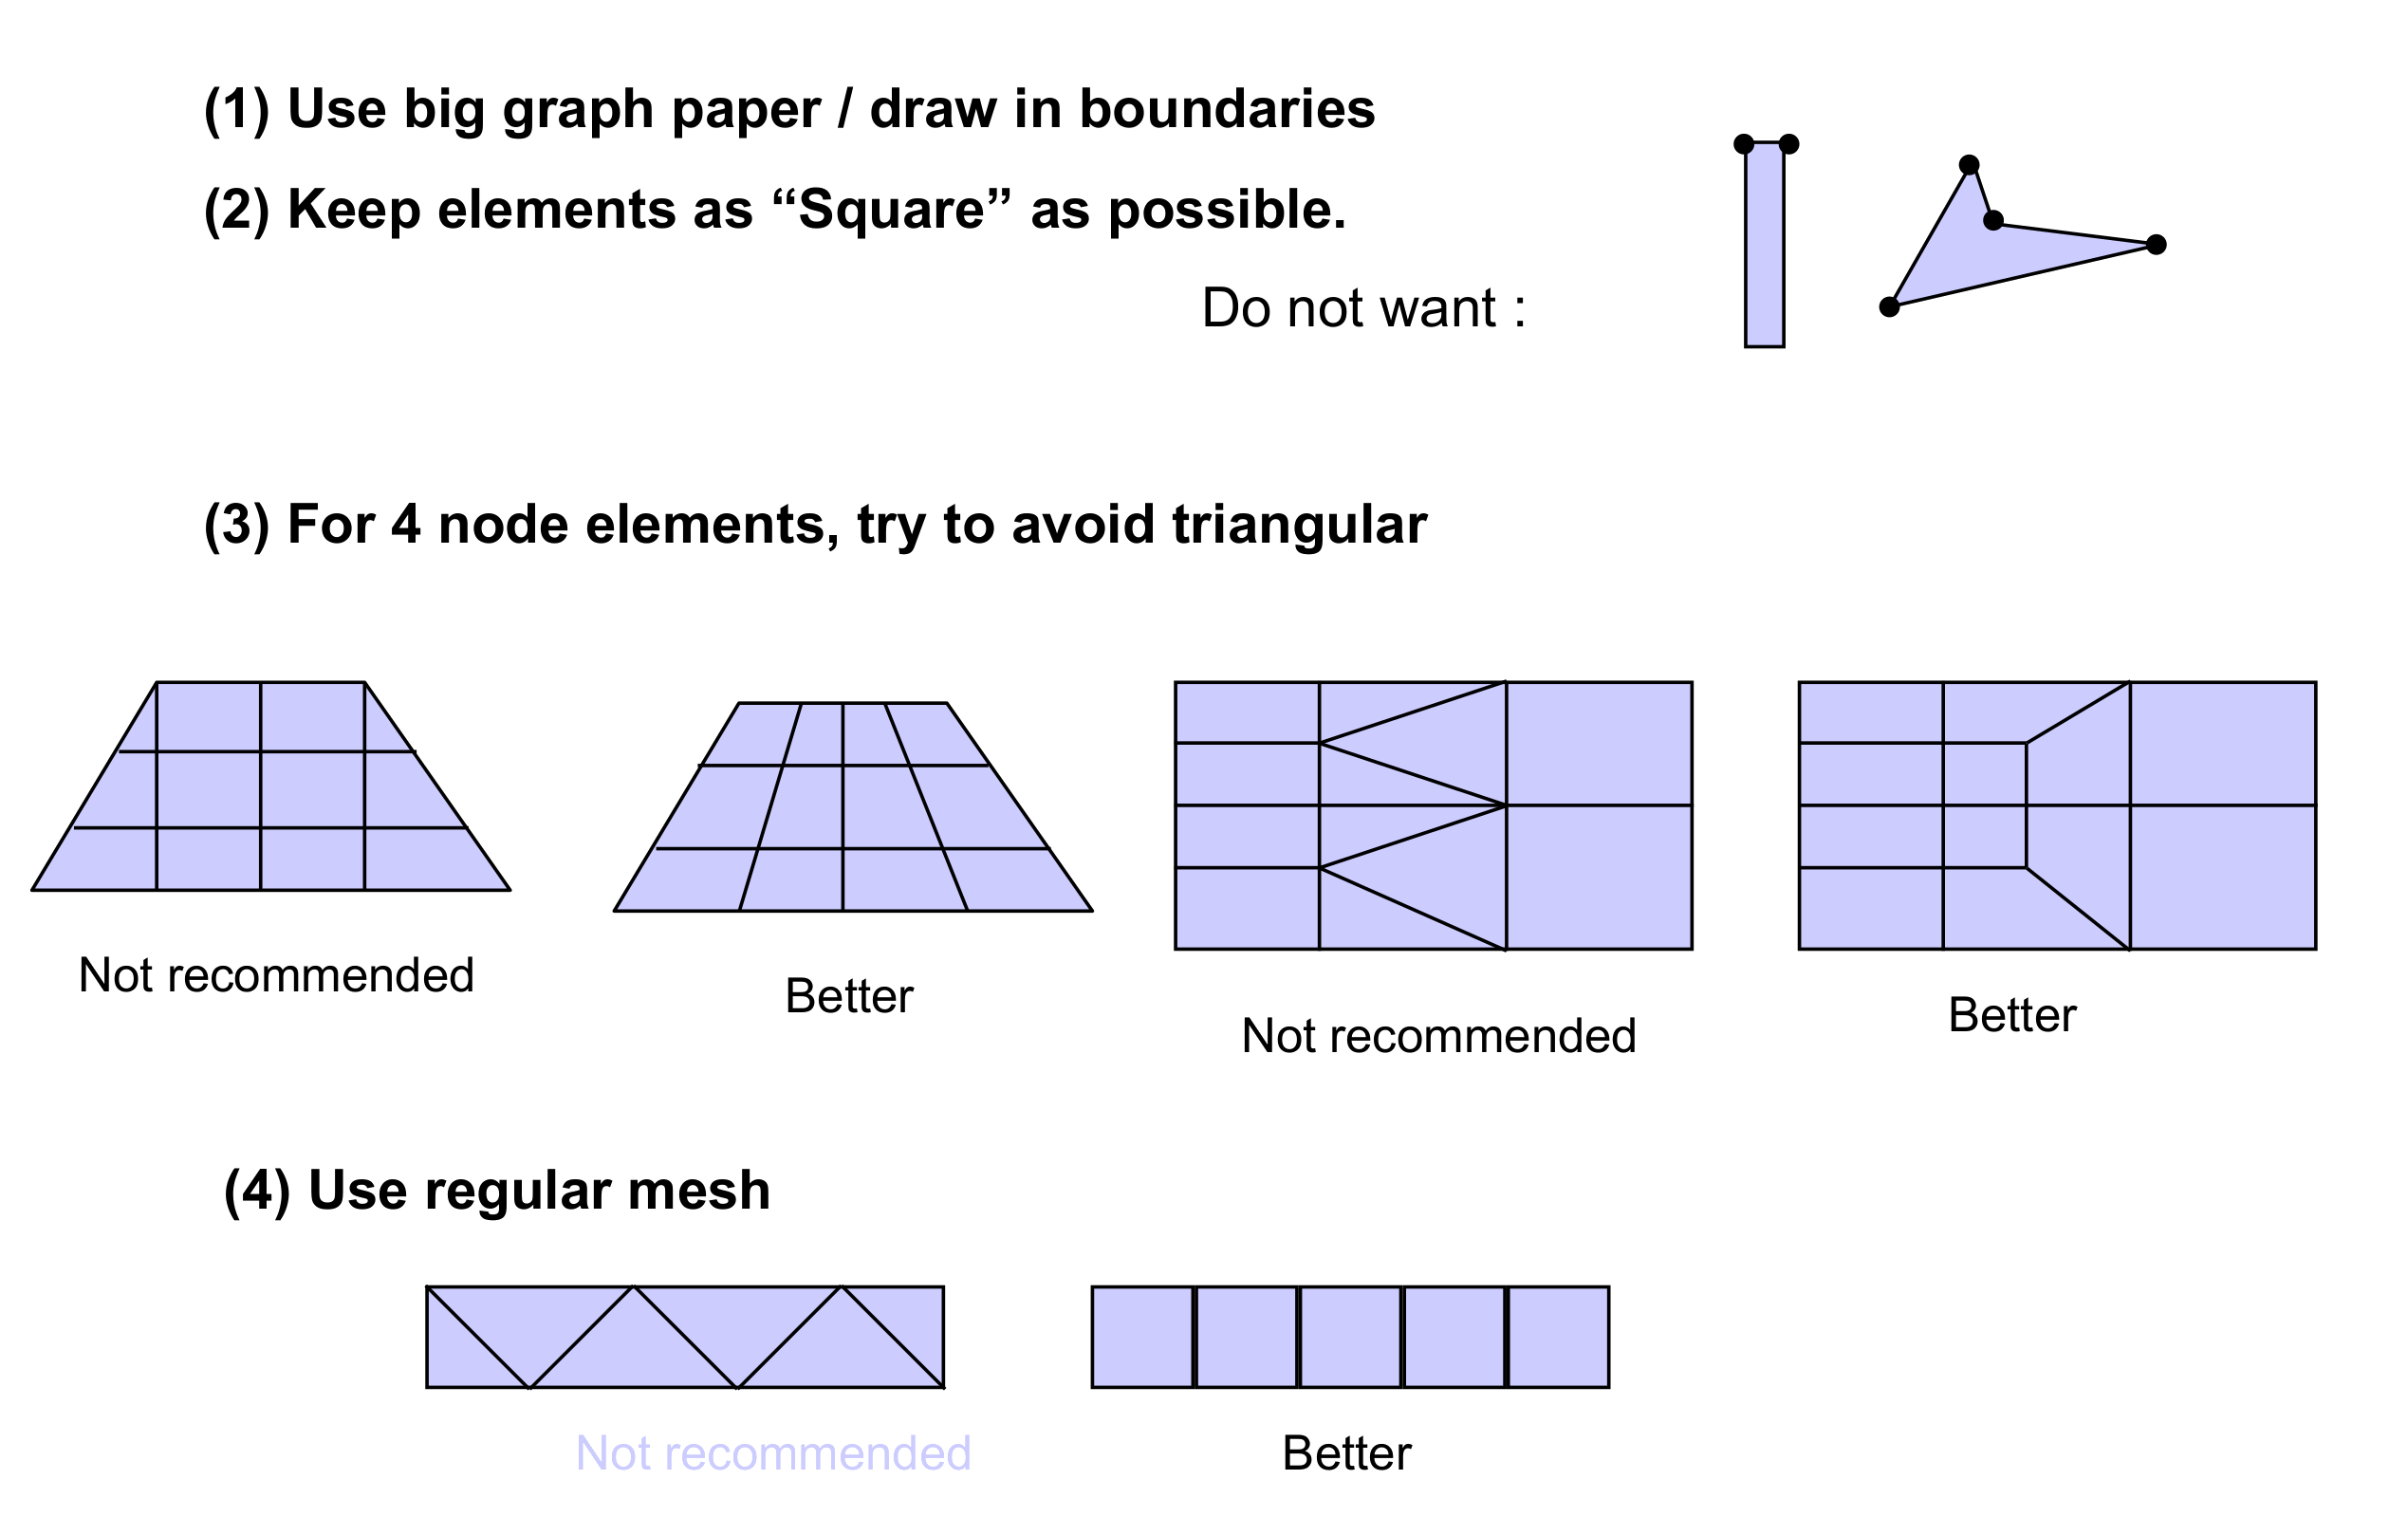
\includegraphics[width=\textwidth]{figs/fe-elements.png}
	\end{figure}
}
\mode<handout>{
	\begin{figure}[ht]
		\centering
		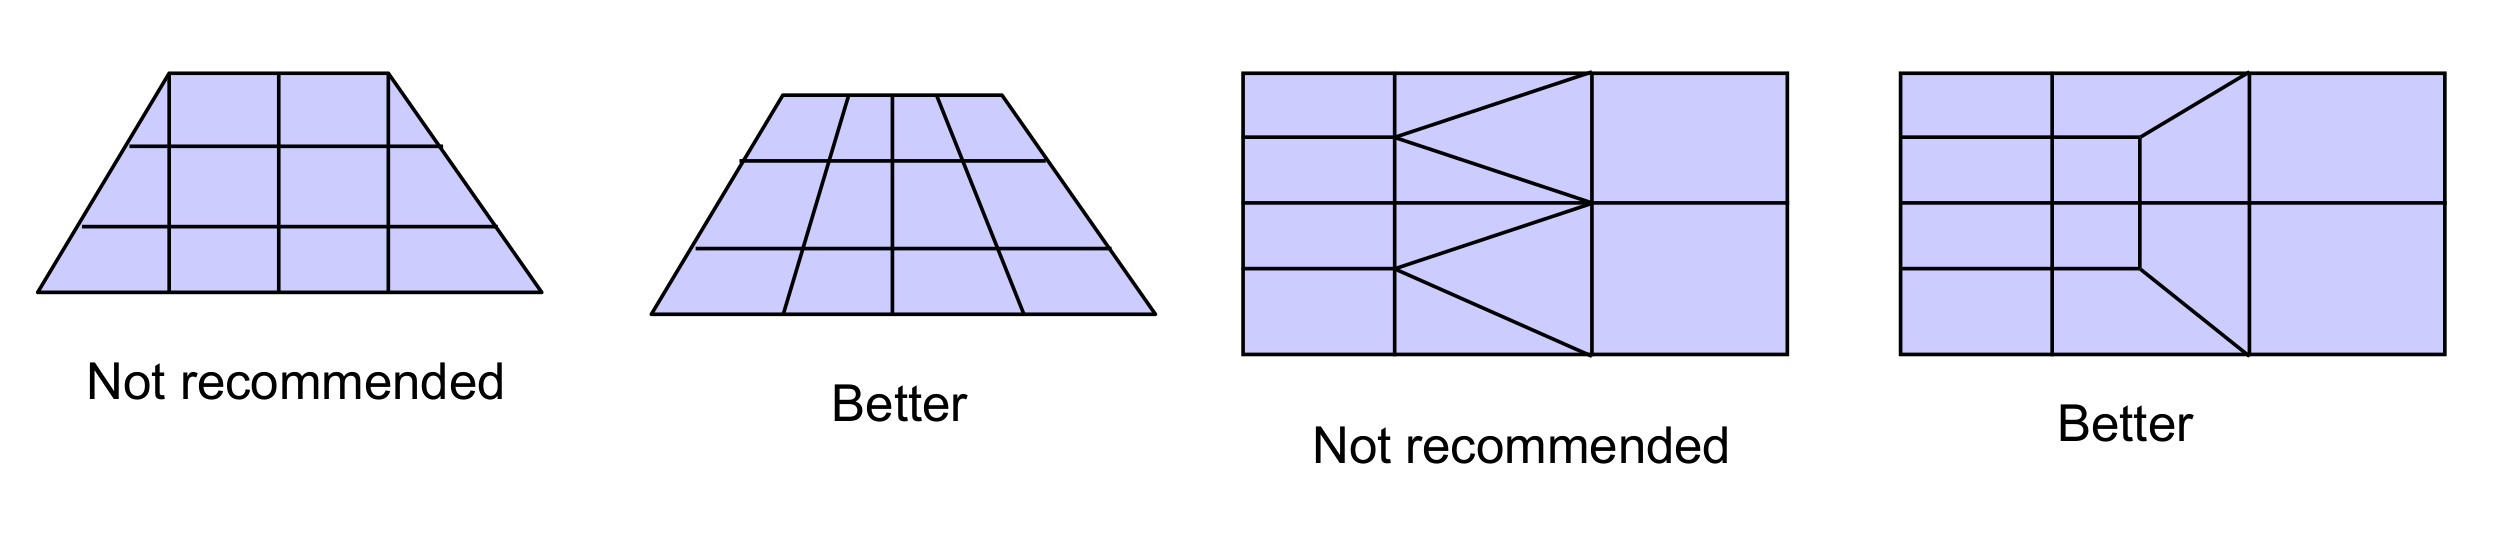
\includegraphics[width=\textwidth]{figs/good-fe-elements.png}
	\end{figure}
	\vspace{4cm}
}
\end{frame}

%------------------------------------------------
\begin{frame}
\frametitle{FE discretization: Refining}
\begin{figure}[ht]
	\centering
	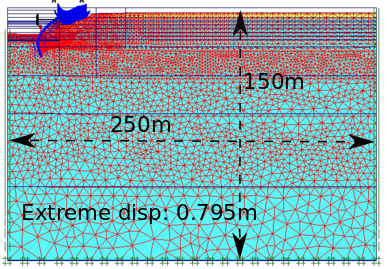
\includegraphics[width=0.8\textwidth]{figs/refined-mesh.png}
	\caption*{Avoid large jumps in element size: size jump should be $< 3$}
\end{figure}
\end{frame}

\subsection{Boundary conditions}
%------------------------------------------------
\begin{frame}
\frametitle{FE boundary conditions}
\begin{figure}[ht]
	\centering
	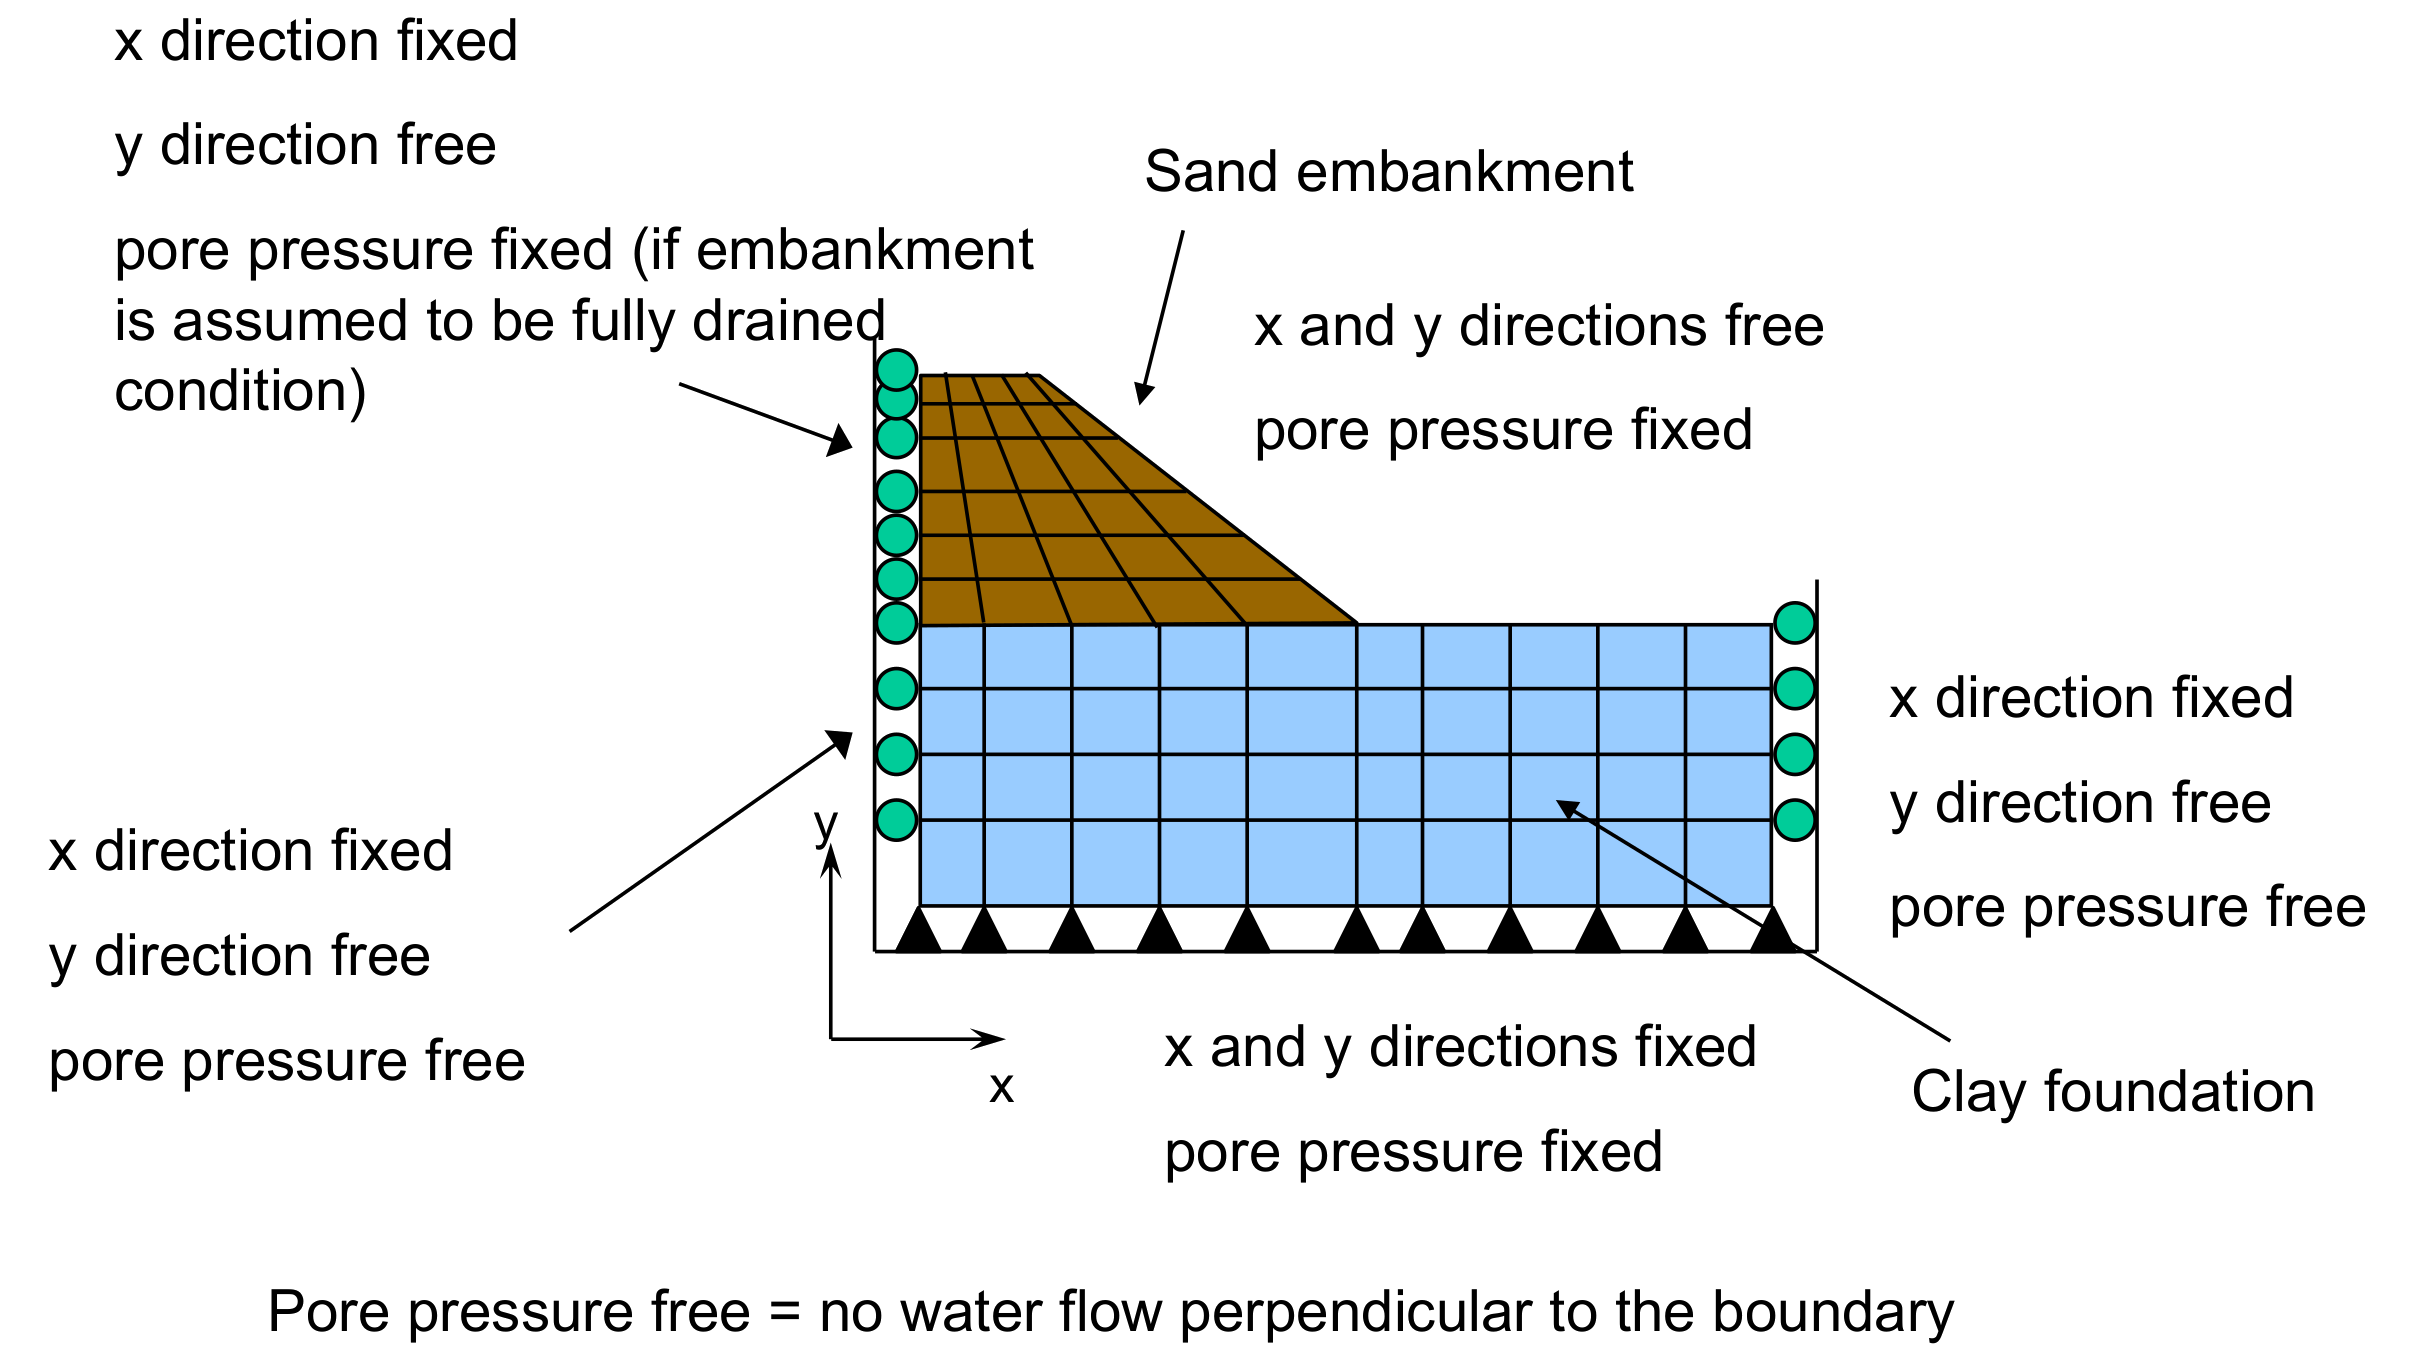
\includegraphics[width=\textwidth]{figs/boundary-conditions.png}
\end{figure}
\end{frame}

%------------------------------------------------
\begin{frame}
\frametitle{FE boundary conditions}
\begin{figure}[ht]
	\centering
	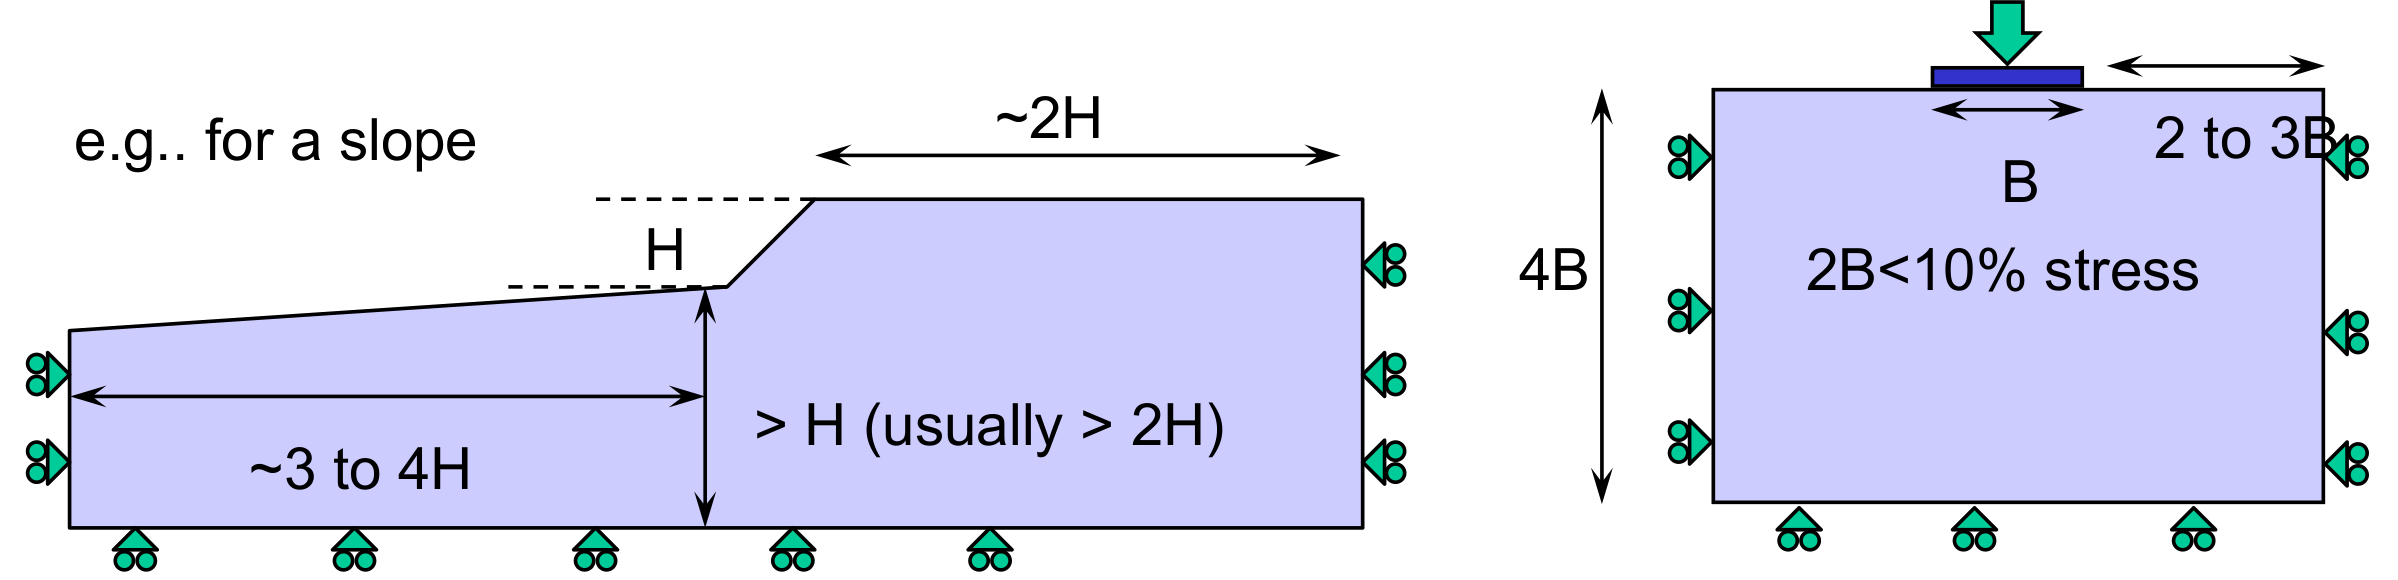
\includegraphics[width=\textwidth]{figs/fe-boundaries.png}
\end{figure}
\end{frame}

\subsection{Errors in FEA}
%------------------------------------------------
\begin{frame}
\frametitle{FE errors}
\mode<beamer>{
	\begin{figure}[ht]
		\centering
		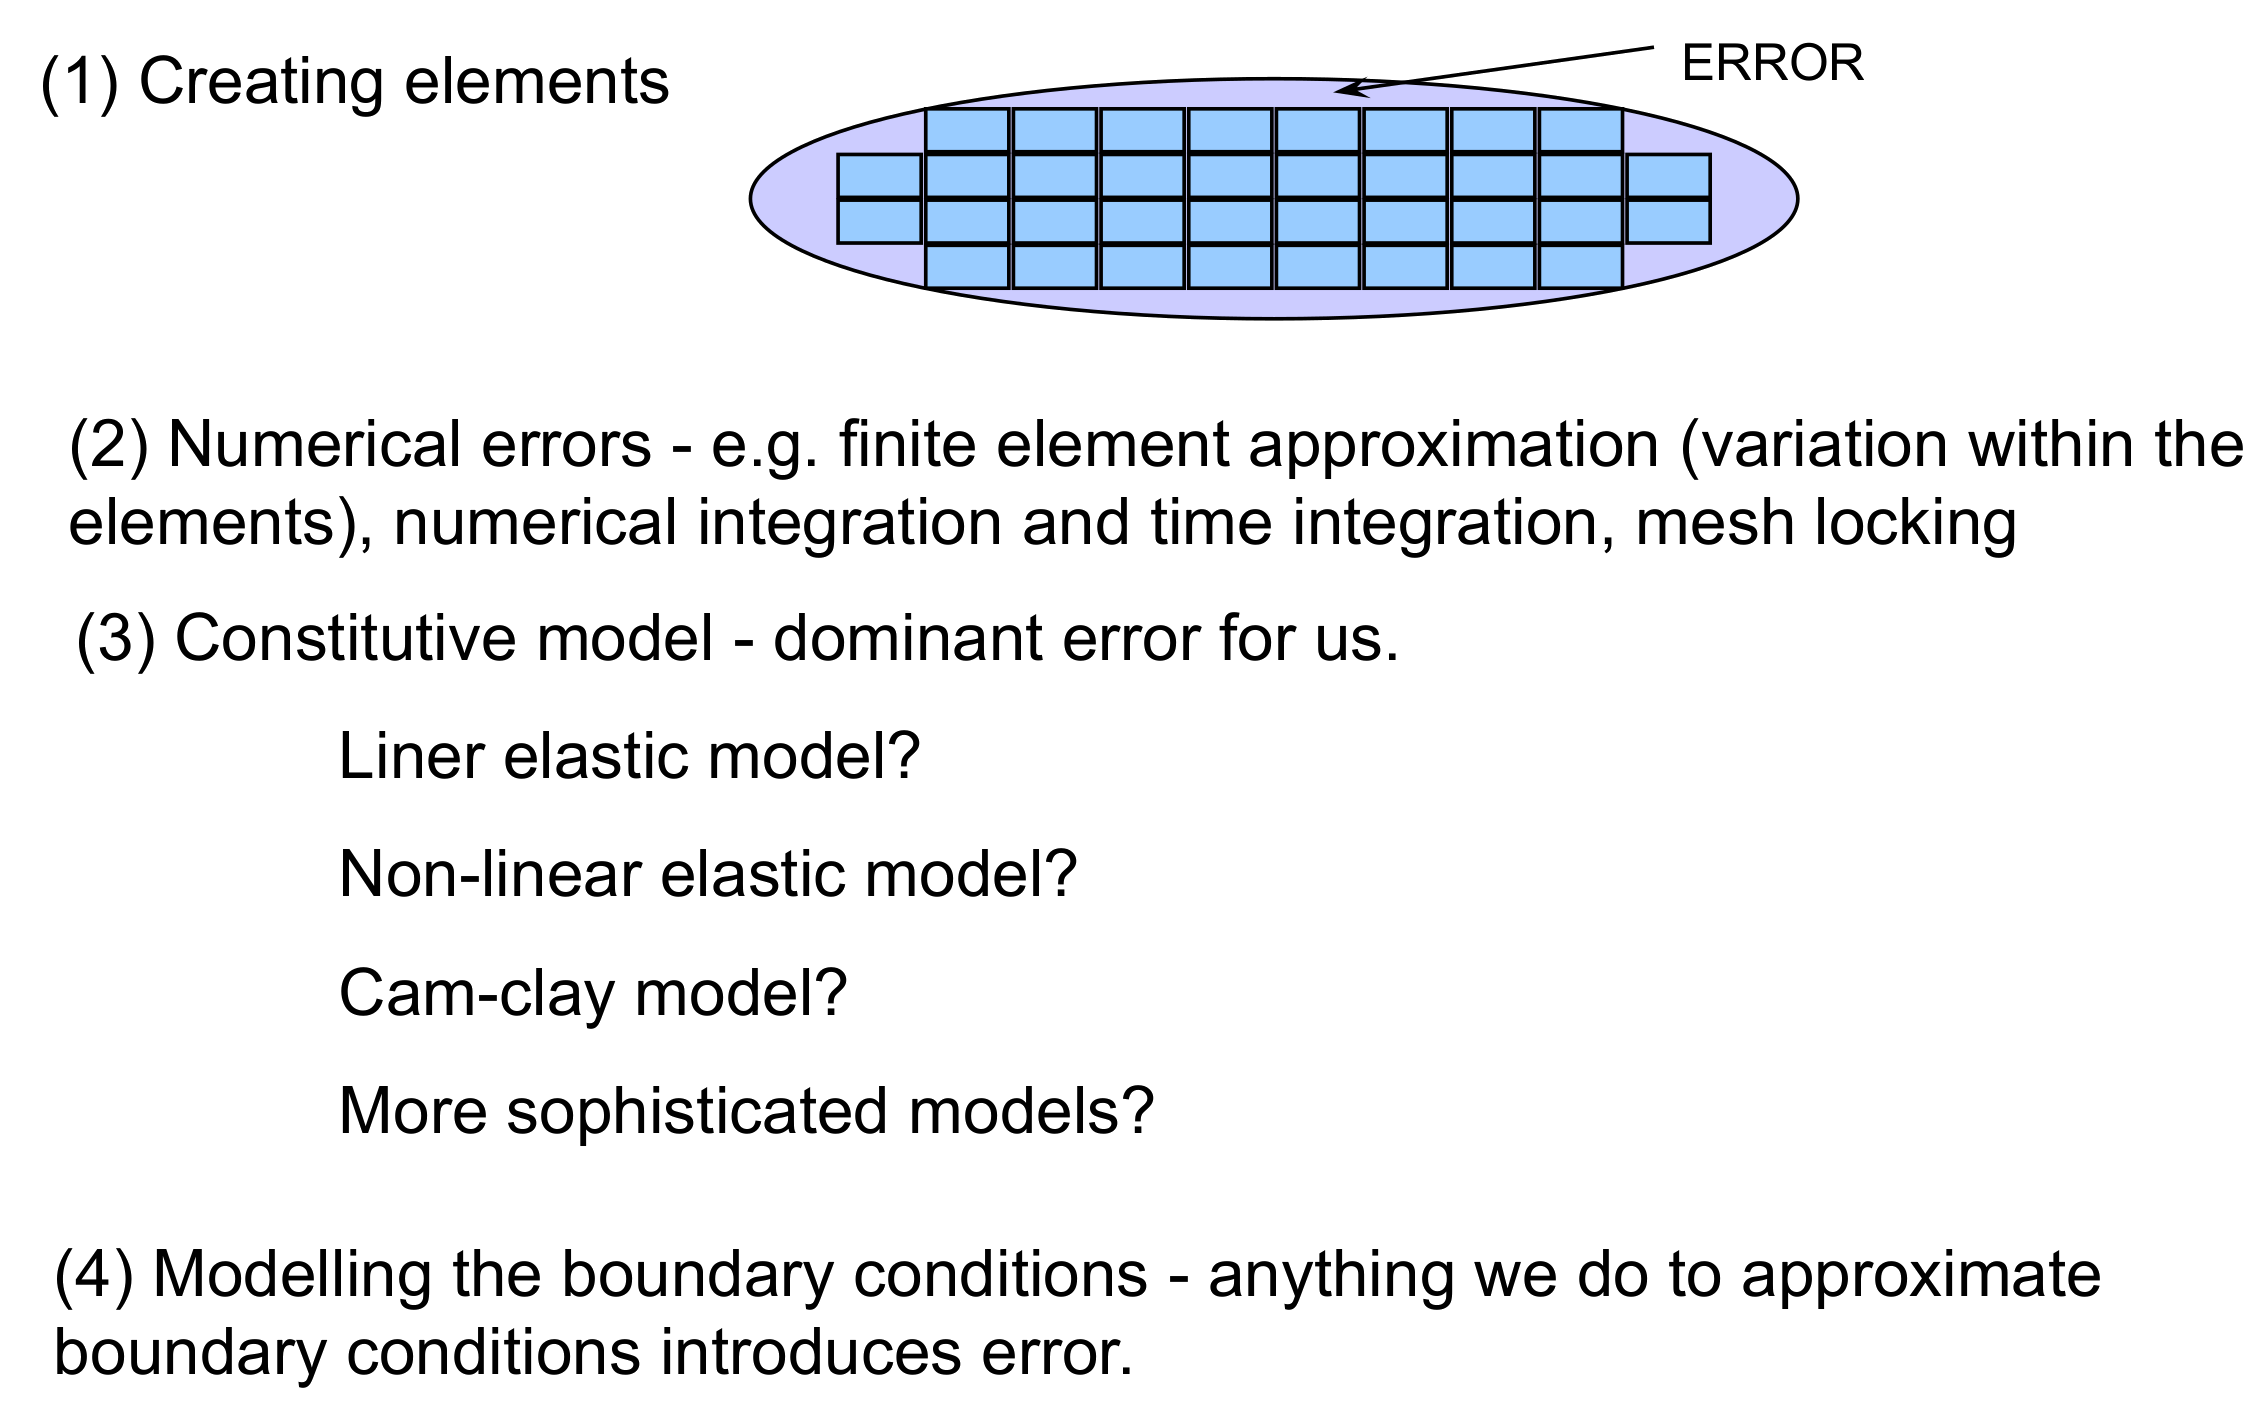
\includegraphics[width=0.9\textwidth]{figs/fe-errors.png}
	\end{figure}
}
\mode<handout>{
	\vspace{6cm}
}
\end{frame}

%------------------------------------------------
\begin{frame}
\frametitle{Undrained analysis}
\mode<beamer>{
	\begin{itemize}
		\item Method A and Method B refers to 2 alternatives modeling of undrained behaviour in Plaxis. 
		\item \textbf{Method A is an effective stress analysis} of an undrained problem it assumes an isotropic elastic behavior and a Mohr-Coulomb failure criterion. 
		\item As a result mean effective stress $p^\prime$ is constant until yield.
		\item Method A was being applied to marine clays which were of low over-consolidation or even under-consolidated because of recent reclamation.
	\end{itemize}
}
\mode<handout>{
	\vspace{6cm}
}
\end{frame}

%------------------------------------------------
\begin{frame}
\frametitle{Undrained effective stress analysis}
\mode<beamer>{
	\begin{figure}[ht]
		\centering
		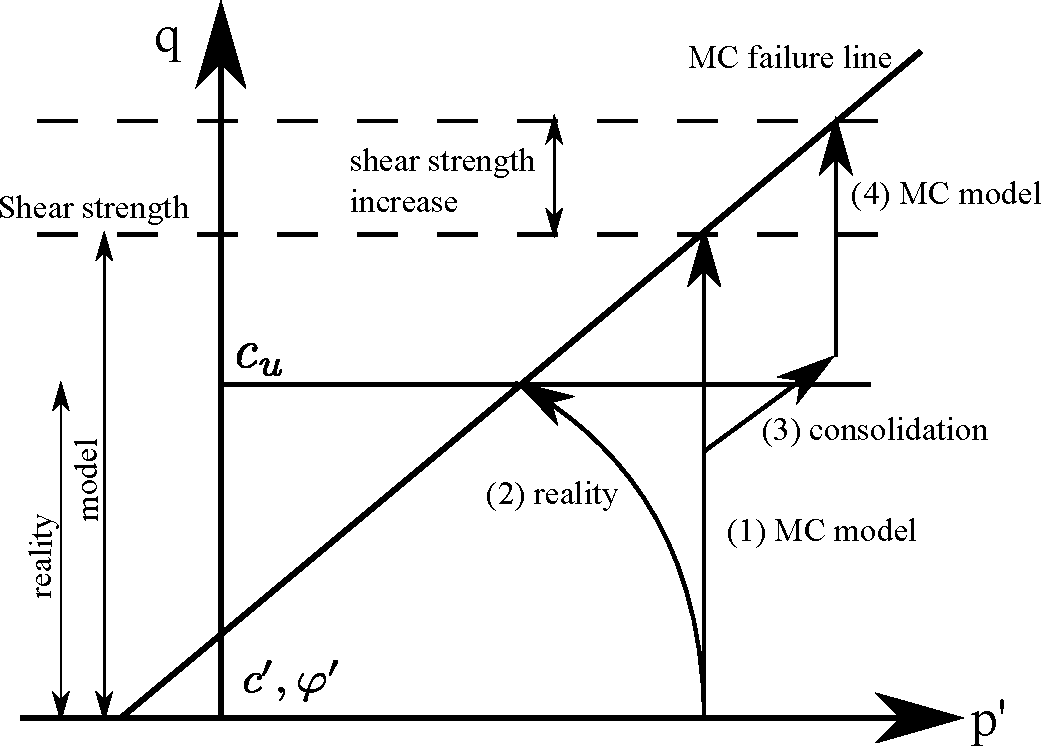
\includegraphics[width=0.75\textwidth]{figs/mc_undrained}
	\end{figure}
}
\mode<handout>{
	\vspace{6cm}
}
\end{frame}

\note{
\textbf{Discuss the effect of depth on the increase in shear strength}
	\begin{figure}
		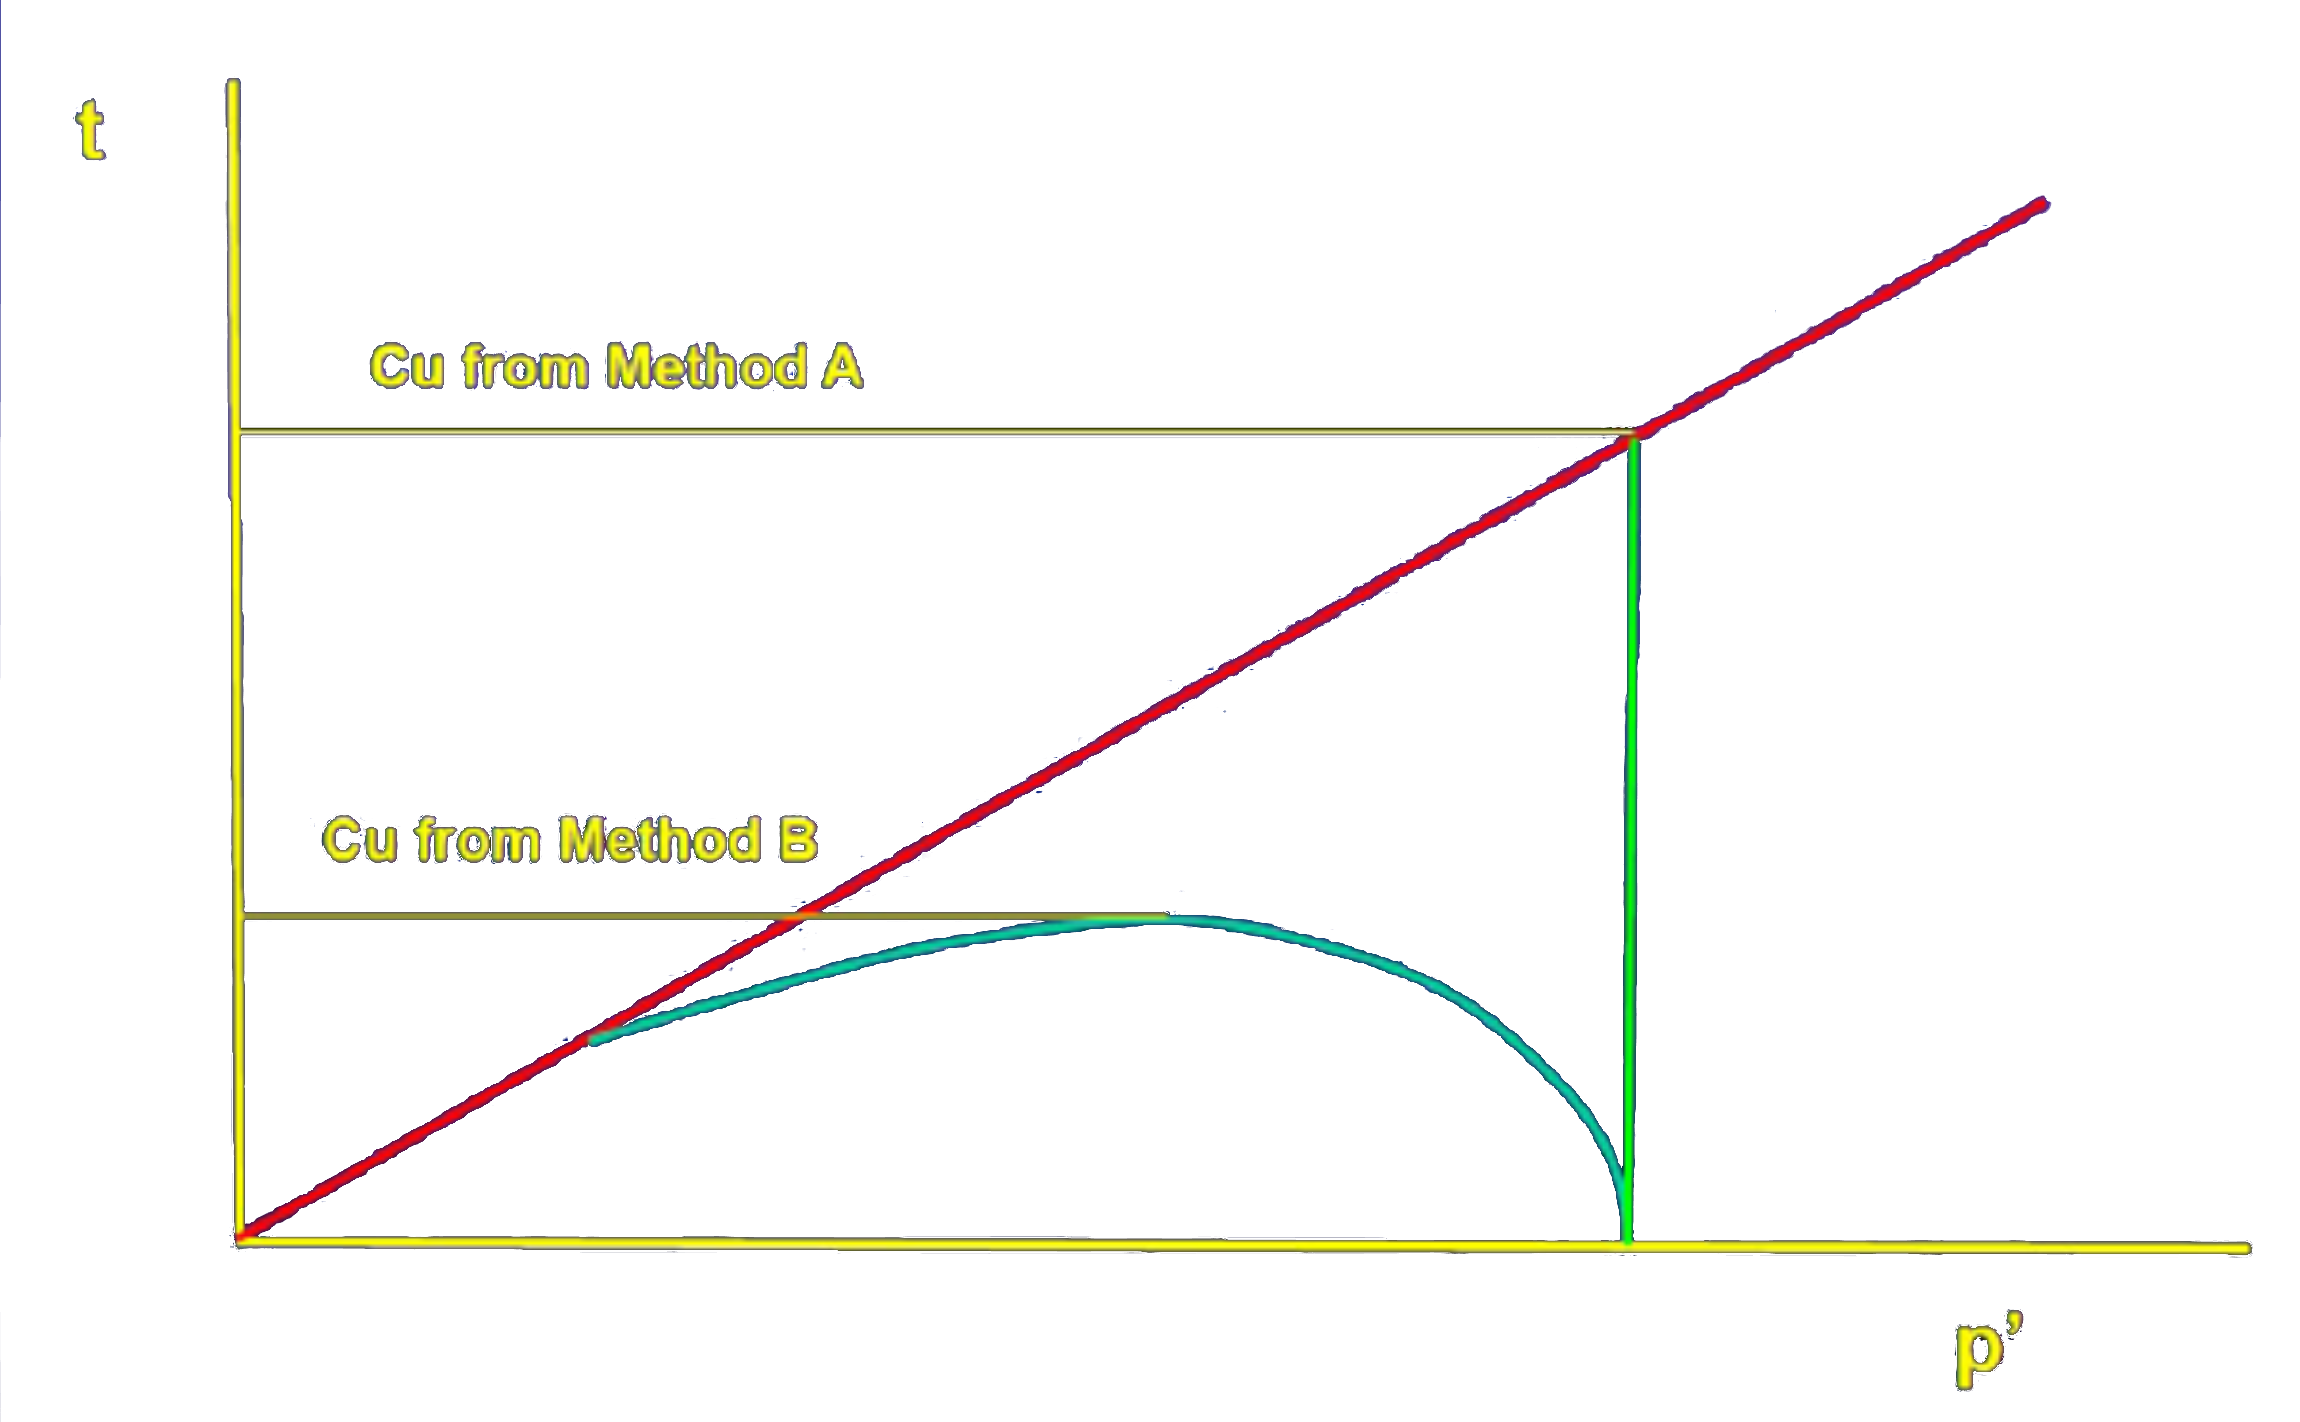
\includegraphics[width=0.6\textwidth]{figs/cu-method-a-b.png}
	\end{figure}
}

%------------------------------------------------
\begin{frame}
\frametitle{Wall displacements: Effective stress vs Undrained strength}
\begin{figure}[ht]
	\centering
	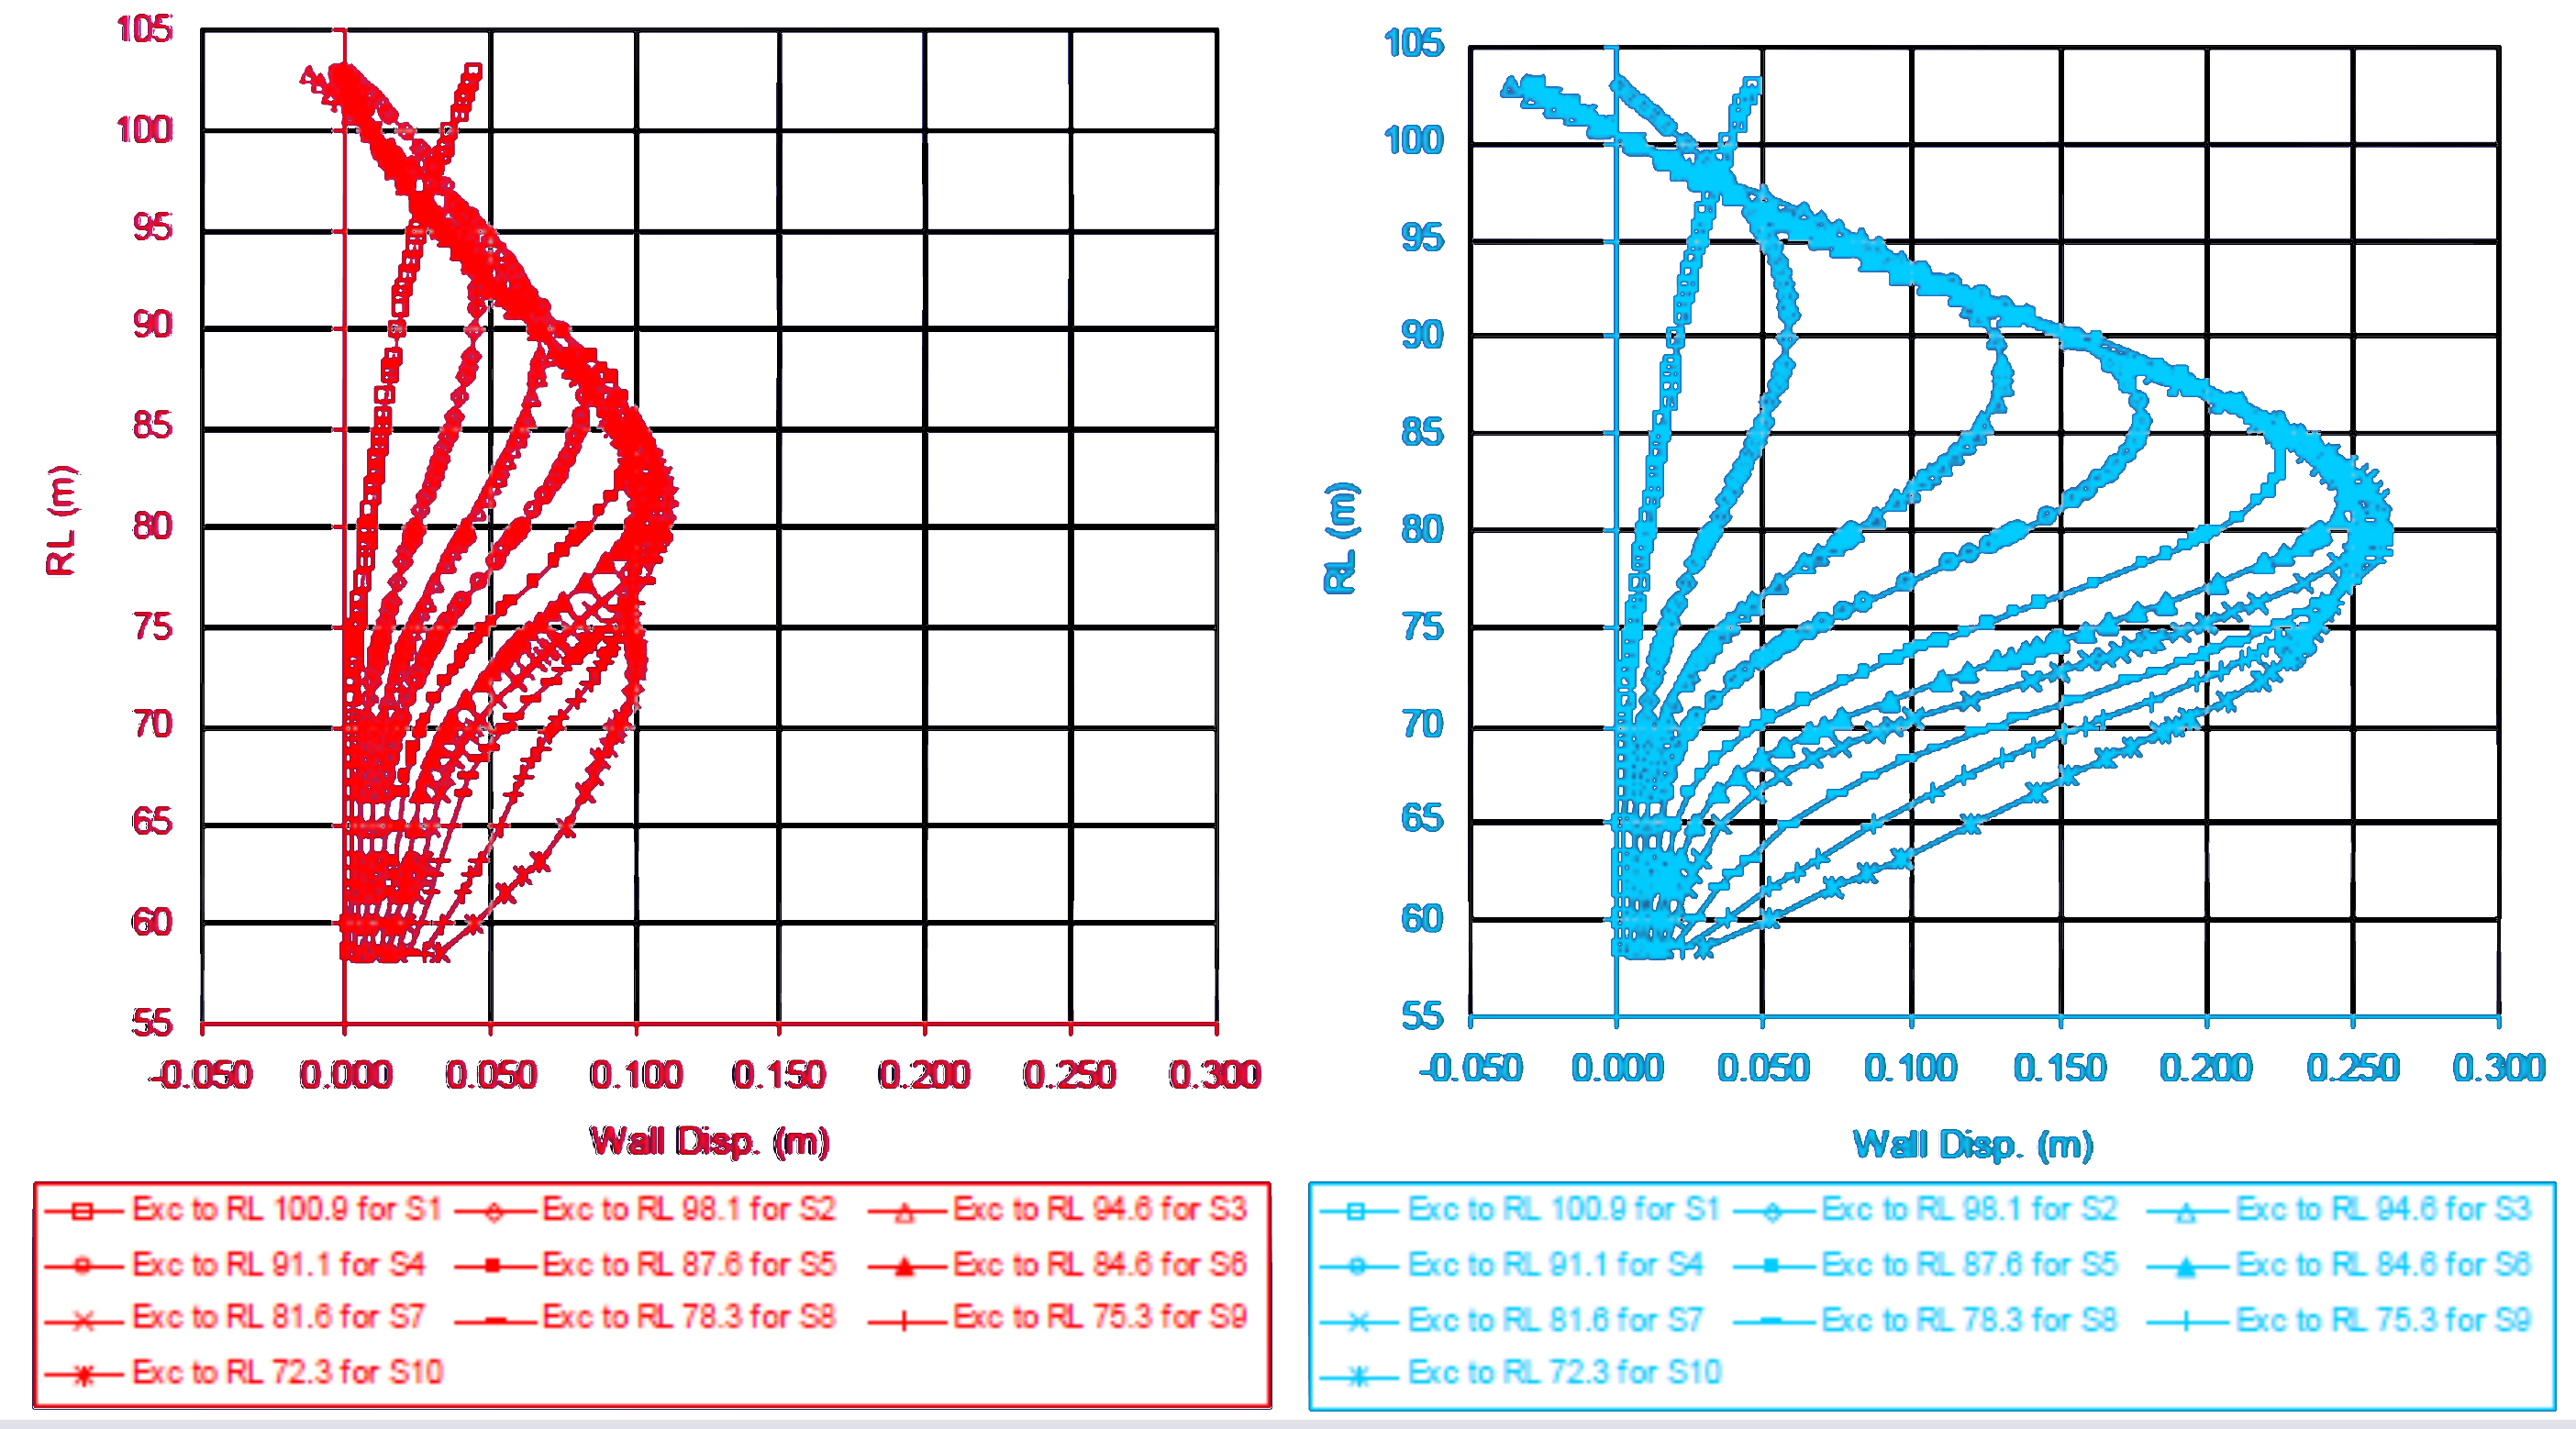
\includegraphics[width=\textwidth]{figs/wall-disp.png}
	\caption*{Nicoll Highway Collapse: Method A vs Method B}
\end{figure}
\end{frame}

%------------------------------------------------
\begin{frame}
\frametitle{Bending moments: Effective stress vs Undrained strength}
	\begin{figure}[ht]
		\centering
		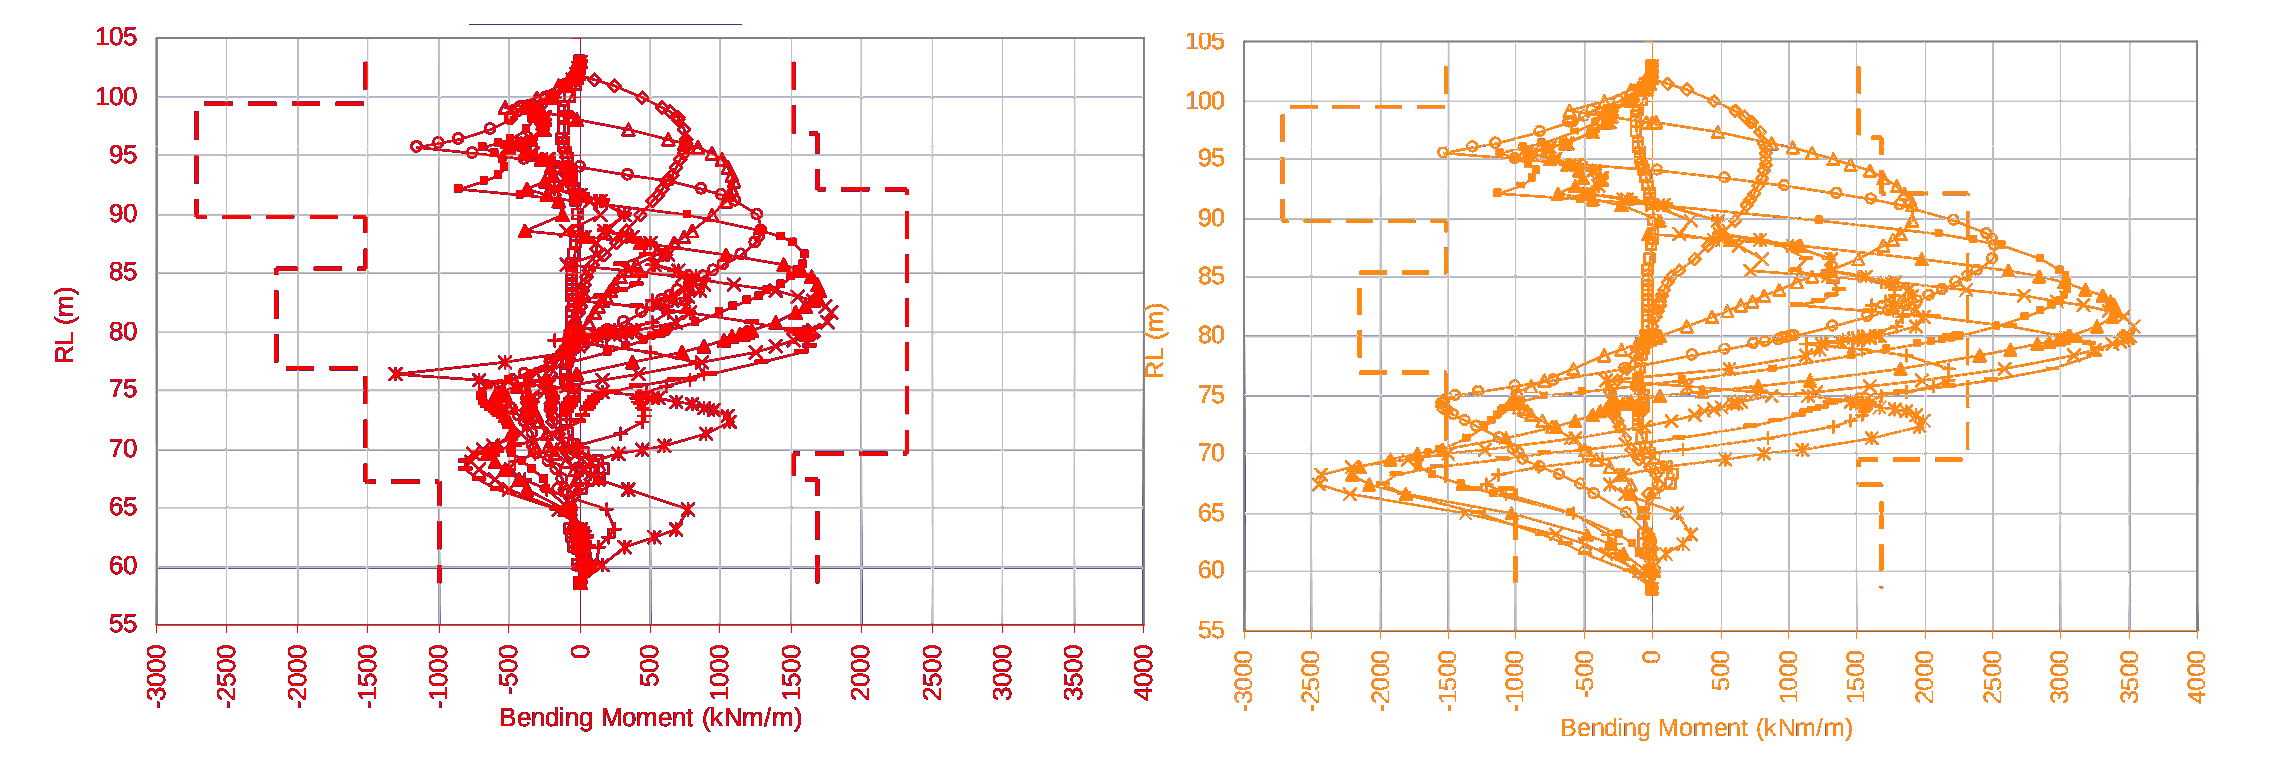
\includegraphics[width=\textwidth]{figs/bending-moments.png}
		\caption*{Nicoll Highway Collapse: Method A vs Method B}
	\end{figure}
\end{frame}


\end{document}